% Created 2014-08-30 Sat 15:30
\documentclass{article}
\usepackage[utf8]{inputenc}
\usepackage[T1]{fontenc}
\usepackage{fixltx2e}
\usepackage{graphicx}
\usepackage{longtable}
\usepackage{float}
\usepackage{wrapfig}
\usepackage{soul}
\usepackage{textcomp}
\usepackage{marvosym}
\usepackage{wasysym}
\usepackage{latexsym}
\usepackage{amssymb}
\usepackage{geometry}
\usepackage{rotating}
\usepackage{hyperref}
\tolerance=1000
\usepackage[margin=1in]{geometry}
\usepackage[round]{natbib}
\usepackage[nonumberlist]{glossaries}
\usepackage[inline]{enumitem}
\setlist{nolistsep}
\usepackage{graphicx}
\usepackage{pdflscape}
\usepackage{multicol}
\newglossaryentry{pc}{name={PC}, description={Pitch Class}}
\newglossaryentry{pcset}{name={PC-Set}, description={Pitch Class Set}}
\newglossaryentry{sc}{name={SC}, description={Set Class}}
\newglossaryentry{nc}{name={nC}, description={Cardinality Class}}
\newglossaryentry{hashnc}{name={\#nC}, description={Size of nC}}
\newglossaryentry{ic}{name={IC}, description={Interval Class}}
\newglossaryentry{tnx}{name={Tn(X)}, description={Transposition}}
\newglossaryentry{ix}{name={I(X)}, description={Inversion}}
\newglossaryentry{tntype}{name={Tn-Type}, description={Transpositional SC-type}}
\newglossaryentry{itype}{name={I-Type}, description={Inversional SC-Type}}
\newglossaryentry{tnitype}{name={TnI-Type}, description={Transpositional/Inversional SC-Type}}
\newglossaryentry{primeform}{name={Prime Form}, description={PC-set representing all members of an SC}}
\newglossaryentry{icv}{name={ICV}, description={Interval-class Vector}}
\newglossaryentry{ncv}{name={nCV}, description={n-class subset vector}}
\newglossaryentry{ncpv}{name={nC\%V}, description={n-class subset percentage vector}}
\newglossaryentry{nsatv}{name={nSATV}, description={n-class subset saturation vector}}
\newglossaryentry{dv}{name={DV}, description={Difference Vector}}
\newglossaryentry{hashx}{name={\#X}, description={Set cardinality}}
\newglossaryentry{hashncv}{name={\#nCV}, description={Vector cardinality}}
\newglossaryentry{trivialform}{name={Trivial Form}, description={SCs 1-1, 11-1 and 12-1}}
\makeglossaries
\providecommand{\alert}[1]{\textbf{#1}}

\title{\Huge \bf Evaluation of Set Class Similarity Measures for Tonal Analysis}

\author{\LARGE Nicholas Harley\\ \\ \LARGE SMC Masters Thesis\\ \\ \LARGE Supervisor: Agust\a'in Martorell}
\date{\today}
\hypersetup{
  pdfkeywords={},
  pdfsubject={},
  pdfcreator={Emacs Org-mode version 7.9.3f}}

\begin{document}

%\maketitle
\begin{centering}
\newgeometry{left=0cm,right=0cm,top=0cm,bottom=0cm}

\includegraphics[width=1\linewidth]{./head.png}
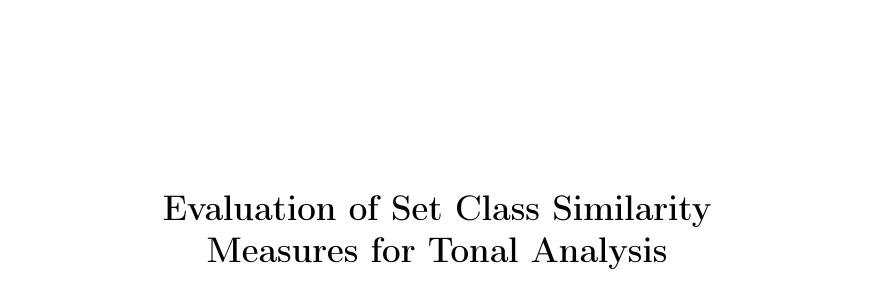
\includegraphics[width=1\linewidth]{./title.png}

\includegraphics[width=1\linewidth]{./space.png}

\includegraphics[width=1\linewidth]{./author.png}
\restoregeometry
\end{centering}

\clearpage

\newgeometry{top=10cm,bottom=2.25cm}
\begin{abstract}

This work explores the limitations of exiting approaches to
computational modelling and description of tonality. Set class 
theory is presented as alternative or complement to existing
approaches. Set class similarity is presented as a tool for
the representation of set class information for structural analysis. 
A survey of set class similarity measures from the literature is 
conducted as well as a rendering of traditional musicological terminology in the language 
of set class theory. Six of the most suitable measures are chosen for 
further evaluation. An analysis methodology is outlined which emphasises systematicity 
and perceptual relevance. This methodology consists of a number of computational techniques 
and is used to analyse specific musical examples. The analytical potential of 
the similarity measures is evidenced through the reconstruction of basic 
music intuition and analysis using the proposed methodology.

\end{abstract}

\clearpage
\newgeometry{top=2.25cm,bottom=2.25cm}

\setcounter{tocdepth}{3}
\tableofcontents
\vspace*{1cm}


\clearpage
\listoftables
\clearpage
\glsaddall
\printglossary[title=Set Class Theory Glossary]
\clearpage
\section{Introduction}
\label{sec-1}

The objectives of the present work are principally concerned with
descriptive modelling of tonality using set class theory. In
particular, the analytical potential of set class similarity measures
will be assessed and evaluated through practical demonstration within
a specific methodological framework. The tentative goal, therefore, is
to present this approach in such a way as to make it relevant to the
wider community of music researchers, such as those in MIR.
\subsection{Problem}
\label{sec-1-1}

\begin{enumerate}
\item Existing computational description of tonality is often limited in
   its scope.
\item The predominant use of template matching for chord and key
   estimations limits the knowledge of music-capable systems to
   repertoire of the major-minor paradigm. This narrow view of
   tonality is insufficient for even some western music.
\item The predominant use of non-musical similarity measures in MIR such
   as Euclidean distance and correlation seems counter-intuitive in
   many cases.
\item The above may be contributing to the ``semantic gap''.
\end{enumerate}
\subsection{Objectives}
\label{sec-1-2}

\begin{enumerate}
\item To adopt a systematic approach to description of tonality.
\item To justify set class analysis as a systematic descriptive tool,
   capable of relating useful musical information as well as having a
   degree of perceptual relevance.
\item To position set class analysis among existing methods of tonal
   description such as chroma vector time-series.
\item To create a comprehensive and practical survey of set class
   similarity measures.
\item To examine the measures in terms of systematicity and perceptual
   relevance.
\item To develop techniques for the representation of set class
   information so as to expose meaningful musicological information.
\item To utilise set class similarity in these representation.
\item To evaluate the utility of these similarity measures through
   exploration of SC information to extract a priori knowledge about
   specific pieces. The analytical potential of the model will be
   evidenced through specific analysis examples.
\end{enumerate}
\subsection{Outline}
\label{sec-1-3}

Part I comprises a concise literature review containing background
information and some basic theory. Chapter \ref{sec-2} addresses the
challenges and problems involved in descriptive modelling of tonality
as a means of justification for the proposed approach. Chapter \ref{sec-3} introduces the basic concepts of set class theory
including set class similarity measures. Chapter \ref{sec-4} gives a basic description of multidimensional scaling
techniques and how they can play a role in set class analysis. Chapter
\ref{sec-5} contains a review of the relevant tonal
models that exist so as to give context work that follows.

Part II contains a description of the contribution of this
work. Chapter \ref{sec-6} contains the outcomes of a
comprehensive survey of set class similarity measures that was carried
out. Chapter \ref{sec-7} presents a number of techniques for
obtaining and representing a set class description of a musical piece
and describes the relationship between parameters involved in the
analysis process. Chapter \ref{sec-8} contains a demonstration
of each computation technique using real musical examples.

Part III presents a summary of the findings and discussion of the work
with Chapters \ref{sec-9} and \ref{sec-10} containing conclusions and
future work respectively.

Part IV contains appendices. Appendix \ref{sec-11}
contains a explanation of each similarity measure from the
literature. Appendix \ref{sec-12} contains
additional information regarding the chosen measures. Appendix \ref{sec-13} contains a set class reference guide for pairing
common musical objects with their corresponding set classes.

\clearpage
\part{Background}
\section{Tonality}
\label{sec-2}
\subsection{Defining Tonality}
\label{sec-2-1}
\subsubsection{General Definition}
\label{sec-2-1-1}

Tonality is a notoriously complex musical phenomenon and numerous
definitions have been proposed from a variety of viewpoints. Perhaps
the most general definition is that provided by \citet{Hyer2013}:
``\ldots{} refers to the systematic arrangements of pitch phenomena and
relations between them.'' Explanations of tonality have been provided
through many different disciplines (acoustics, music theory,
linguistics, cognitive psychology) and a detailed discussion of these
areas is certainly beyond the scope of this work. However, it is
generally agreed that tonality is an abstract cultural and cognitive
construct that can have many different physical representations.
\subsubsection{Babbitt's Domains}
\label{sec-2-1-2}

\citet{Babbitt1965} proposed three domains to categorise different
types of representation of music: acoustic (physical), auditory
(perceived), graphemic (notated). Western music theory provides a
lexicon for describing abstract tonal objects with terms such as note,
chord and key. These objects have a hierarchical relationship and the
meaning of these labels is highly dependent on musical context and the
scale of observation. Musicological descriptions, which constitute the
majority of reasoning about tonaility, reside mainly in the Babbitt's
graphemic domain, although arguably they reflect some aspects of the
other two. Each domain, whilst connected to every other, provides only
a projection of the musical whole and examination of tonality from
just one will most likely result in an incomplete picture. However,
these three domains provide a convenient framework for the discussion
that follows.
\subsection{Modelling Tonality}
\label{sec-2-2}

The challenge of mathematically modelling aspects of tonality has been
approached in numerous ways and from different domains. In the
graphemic domain, musicologists and composers have proposed
theoretical models, attempting to rethink tonal theory from a
mathematical perspective. These models employ different branches of
mathematics such as geometry \citep{Tymoczko2012} or group theory
\citep{Ring2011} to describe harmonic structure. From the auditory
domain, cognitive psychologists have built models of tonal induction
based on perceptual ratings of tonal stimuli \citep{Krumhansl1990}.
\subsubsection{Tonality as Context}
\label{sec-2-2-1}

Many models approach the concept of tonality as a context, within
which the relations and hierarchies of tonal phenomena can be
understood. A sense of tonality can be induced when musical stimuli
resemble some a priori contextual category. For western music of the
major-minor period, key signatures comprise a collection of categories
that give context to the tonal components of
music. \citet{Martorell2013} identifies three important aspects of
tonality as context: dimensionality (the relatedness or ``closeness'' of
categories), ambiguity (reference to two or more categories
simultaneously) and timing (the dynamics of tonal context). He
highlights the importance of a models capability to describe these
aspects. 
\subsubsection{Tonality in MIR}
\label{sec-2-2-2}

The MIR community is primarily concerned with the extraction of tonal
descriptors from audio signals such as chord and key estimates. Most
systems use chroma features as a preliminary step, obtained by mapping
STFT or CQ transform energies to chroma bins. Template matching is
used to compare the chroma vectors to a tonal model (contextual
category) using some distance measure. A commonly used tonal model for
key estimation are the KK-profiles \citep{Krumhansl1990} (\ref{sec-5-3}) (e.g. in \citealt{Gomez2006}). Distance measures such as
inner product (e.g. in \citealt{Gomez2006}) and fuzzy distance
(e.g. in \citealt{Purwins2000}) are used to compare
vectors. Statistical methods, such as HMMs, have been used for chord
and key tracking \citep{Chai2005}. Of addition interest in the field
is the concept of musical similarity (for music recommendation,
structure analysis, cover detection etc.). \citet{Foote2000} computed
self-similarity matrices for visualisation of structure by correlating
the MFCC feature vector time-series. \citet{Gomez2006} proposed the
application of this method to tonal feature vectors.
\subsubsection{Similarity}
\label{sec-2-2-3}

The importance of defining the similarity or closeness between musical
phenomena, be it theoretical, physical or perceptual, is central to
almost every model of tonality and often leads to a geometric
configuration of tonal objects. The concepts of similarity and
distance is discussed further in Chapter \ref{sec-5}
where a review of spatial models of tonality is given.
\subsection{The Semantic Gap}
\label{sec-2-3}
\subsubsection{Acoustic Domain}
\label{sec-2-3-1}

\citet{Wiggins2009} discusses, what is referred to in MIR as, the
``Semantic Gap'': the inability of systems to achieve success rates
beyond a conspicuous boundary. He examines the fundamental
methodological groundings of MIR in terms of Babbitts three domains,
discussing the limits of each representation and regarding the
discarnate nature of music. He concludes that the audio signal
(acoustic domain) simply cannot contain all of the information that
systems seek to retrieve. He points towards the the auditory domain as
the chief residence of music information and urges for in not to be
overlooked in MIR and wider music research.
\subsubsection{Graphemic Domain}
\label{sec-2-3-2}

Furthermore, Wiggins criticises the purely graphemic approach and the
tendency of music research to presuppose musicological
axioms. \citet{Wiggins2012} argues that music (tonal) theory is,
rather than a theory in the scientific sense, a highly developed folk
psychology (internal human theory for explaining common
behaviour). Thus, the rules of music theory are not like scientific
laws but rather abstract descriptions of a specific musical
behaviour. This idea challenges the validity of formalising such rules
in mathematics and prompts the question, ``What is actually being
modelled?'' He concludes that to apply mathematical models to musical
output alone (scales or chords) without consideration of the musical
mind is a scientific failure.
\subsubsection{Problems}
\label{sec-2-3-3}

The two assertions of Wiggins sit contrary to a number of the aspects
of the tonal models discussed in \ref{sec-2-2}. Firstly, the
major-minor paradigm, upon which many systems are based, whilst
certainly possessing perceptual significance, is still a musicological
concept and therefore a misleading basis for both mathematical and
cognitive approaches. A second problem is that of the numerical
methods used by some MIR systems, in particular, distance measures. As
will be discussed in Chapter \ref{sec-5}, similarity
(and by extension distance) is a central part of the auditory
domain. MIR systems often uses distance measures from mathematics such
as Mahalanobis \citep{Tzanetakis1999} or Cosine \citep{Foote2000} with
little consideration of their perceptual or musical significance.
\subsection{Systematicity}
\label{sec-2-4}
\subsubsection{The Musical Surface}
\label{sec-2-4-1}

Having cautioned against a purely musicological approach,
\citet[pp. 481]{Wiggins2009} proposes a compromise: to adopt a
bottom-up approach to music theory, exploring the concepts through
systematic mid-level representations. He states that ``methods
starting at, for example, the musical surface of notes is a useful way
of proceeding'' The concept of musical surface is illustrated by
\citet[pp. 159]{Huovinen2007} with a metaphor: ``\ldots{}to approach a
musical landscape not by drawing a map, which necessarily confines
itself to a limited set of structurally important features, but by
presenting a bird’s-eye view of the musical surface – an aerial
photograph, as it were, which details the position of every pitched
component.''
\subsubsection{Systematic Description}
\label{sec-2-4-2}

\citet{Martorell2013} also advocates this mid-level approach,
observing that surface description influences analytical observation
and that, for an unbiased view, the researcher must be provided with
the adequate raw materials with which to make more in-depth
observation. Such a systematic, descriptive model would be
fundamentally independent of high level concepts such as chords and
key but, at the same time, capable of capturing
them. \citet{Martorell2013} also discusses the importance of
systematicity in terms of dimensionality, ambiguity and timing. He
finds that models based on the major-minor paradigm are incapable of
adequately describing tonal ambiguity even in some Western music
\citep[chap. 3]{Martorell2013}.

With a systematic description of the musical surface, theories and
models from different domains can be gathered and evaluated together in
the same analytical arena, thus helping to bridge the gap between
traditional musicology, cognitive psychology and MIR.

\section{Set Class Theory}
\label{sec-3}

One such method available for systematic description of the musical
surface is set class theory. Set class theory is a system for
analysing the pitch content of music. It uses class equivalence
relations to reduce the amount of data required to describe any
collection of pitches. This chapter will outline the basic principles.
\subsection{Pitch Class Set}
\label{sec-3-1}

Set class theory uses octave equivalence. In Western equal temperament
(TET), a pitch class (PC) is an integer representing the residue class
modulo 12 of a pitch \citep(Babbitt1965) and indicates the position of
a note within the octave. A PC-set is a collection of PCs ignoring any
repetitions and the order in which they occur. PC-sets are notated as
follows \{0,1,2,3,4\} with PCs ordered from lowest to highest as a
convention (Example 1). The cardinality of a set, denoted \#S, is the
number of PCs it contains (Example 2). There are 4096 (2$^{\mathrm{12}}$) unique
PC-sets with which any segment of music can be represented.

\begin{table}[htb]
\caption{Notes and corresponding pitch-classes} 
\begin{center}
\begin{tabular}{lrrrrrrrrrrrr}
 Note  &  C  &  C\#  &  D  &  D\#  &  E  &  F  &  F\#  &  G  &  G\#  &  A  &  A\#  &   B  \\
 PC    &  0  &    1  &  2  &    3  &  4  &  5  &    6  &  7  &    8  &  9  &   10  &  11  \\
\end{tabular}
\end{center}
\end{table}



\begin{center}
\begin{tabular}{llll}
 Example 1:  &  PC-set       &  Pitch-set  &  S = \{A4,C5,E5,A5\} (A minor)  \\
             &               &  PC-set     &  S = \{9,0,4,9\} = \{0,4,9\}    \\
 Example 2:  &  Cardinality  &             &  \#S = 3                        \\
\end{tabular}
\end{center}
\subsection{Set Classification}
\label{sec-3-2}

Defining equivalence classes of PC-sets further reduces the total
number of tonal objects. A set-class (SC) is a group of PC-sets
related by a transformation or group of transformations. The two types
of transformation commonly used are transposition and inversion. A
transposition, Tn(S), transposes the set, S, by the interval, n, (by
adding n to all PCs, Example 3). An inversion, I(S), inverts the set
S, replacing all PCs with their inverse (12-PC, Example 4). From these
two transformations it is possible to define three types of SC: Tn,
TnI and I.


\begin{center}
\begin{tabular}{lll}
 Example 3:  &  Transposition  &  S = \{0,4,9\}, T3(S) = \{3,7,0\} = \{0,3,7\}   \\
 Example 4:  &  Inversion      &  S = \{0,4,9\}, I(S) = \{11,7,2\} = \{2,7,11\}  \\
\end{tabular}
\end{center}




\begin{center}
\begin{tabular}{ll}
 Transpositional (Tn):  &  All PC-sets that can be transformed to each  \\
                        &  by transposition belong to the same class.   \\
                        &  There are 351 distinct Tn types.             \\
 Inversional (I):       &  All PC-sets that can be transformed to each  \\
                        &  other by inversion belong to the same SC.    \\
                        &  There are 200 distinct I types.              \\
 Transpositional/       &  All PC-sets that can be transformed to each  \\
 Inversional (TnI):     &  other by transposition, inversion or both    \\
                        &  belong to the same SC.                       \\
                        &  There are 223 distinct TnI types.            \\
\end{tabular}
\end{center}



The Prime Form of a PC-set is a convention for denoting the SC it
belongs to. The convention was introduced by Allan Forte
\citep{Forte1973} for TnI types and has since been adopted by the
majority of theorists. In addition, he devised a system for ordering
TnI-type SCs and assigning to each one a cardinality-ordinal
number. For example, the Forte number 3-11 refers to the 11th SC of
cardinality 3. This convention has been modified for use with Tn types
by adding A and B to the names of inversionally related SCs.

One additional concept is that of cardinality-class (nC), which refers
to all the SCs of cardinality n. Cardinality-class 2 is commonly
referred to as interval-class (IC) and there are 6 distinct
interval-classes.
\begin{table}[htb]
\caption{Forte's Prime form and numbering convention} 
\begin{center}
\begin{tabular}{ll}
 PC-set            &  \{0,4,9\}  \\
 Prime Form (TnI)  &  \{0,3,7\}  \\
 Prime Form (Tn)   &  \{0,4,7\}  \\
 Forte Name (TnI)  &  3-11       \\
 Forte Name (Tn)   &  3-11A      \\
\end{tabular}
\end{center}
\end{table}


\begin{table}[htb]
\caption{Numbers of objects} 
\begin{center}
\begin{tabular}{lr}
 Object type  &  No. Objects  \\
\hline
 Pitch        &           88  \\
 Pitch set    &         3e26  \\
 PC           &           12  \\
 PC-set       &         4096  \\
 Tn-Type SC   &          348  \\
 I-Type SC    &          197  \\
 TnI-Type SC  &          220  \\
\end{tabular}
\end{center}
\end{table}


\begin{table}[htb]
\caption{Cardinality Class} 
\begin{center}
\begin{tabular}{lrrr}
      &      &  $\#nC$  &       \\
 n    &  Tn  &       I  &  TnI  \\
\hline
 1C   &   1  &       1  &    1  \\
 2C   &   6  &       6  &    6  \\
 3C   &  19  &      12  &   12  \\
 4C   &  43  &      28  &   29  \\
 5C   &  66  &      35  &   38  \\
 6C   &  80  &      35  &   50  \\
 7C   &  66  &      35  &   38  \\
 8C   &  43  &      28  &   29  \\
 9C   &  19  &      12  &   12  \\
 10C  &   6  &       6  &    6  \\
 11C  &   1  &       1  &    1  \\
 12C  &   1  &       1  &    1  \\
\end{tabular}
\end{center}
\end{table}
\subsection{Vector Analysis}
\label{sec-3-3}
\subsubsection{Membership and Inclusion}
\label{sec-3-3-1}

Two concepts that are crucial in set class theory are membership and
inclusion. Membership of a set is denoted p $\in$ S and means that PC p
is a member of set S (Example 5). Inclusion in a set is denoted Q
$\subset$ S and means that all members of set Q are also members of set
S (Example 6). Q is said to be a subset of S.

\begin{center}
\begin{tabular}{lll}
 Example 5:  &  Membership  &  4 $\in$ \{0,4,9\}                  \\
 Example 6:  &  Inclusion   &  \{0,4,9\} $\subset$ \{0,1,4,5,9\}  \\
\end{tabular}
\end{center}
\subsubsection{Embedding Number}
\label{sec-3-3-2}

\citet{Lewin1979} applied these concepts to SCs to develop his
Embedding Number, EMB(X,Y). Given two SCs, X and Y, EMB(X,Y) is the
number of instances of SC, X, which are included in (are subsets of)
SC, Y (Example 7). X is ring-shifted 11 times and each unique
resulting set which is included in Y adds one to the embedding number.

\begin{center}
\begin{tabular}{lll}
 Example 7:  &  Embedding Number  &  X = \{0,4\} and Y = \{0,4,8\}  \\
             &                    &  so\ldots{} EMB(X,Y) = 3        \\
\end{tabular}
\end{center}
\subsubsection{Subset Vectors}
\label{sec-3-3-3}

An n-class subset vector of X, nCV(X), is an array of values of
EMB(A,X) where A is each of the SCs in the cardinality-class, nC
(Example 8). The Interval-Class Vector (ICV) is a special instance of
the nCV with n equal to 2. Vector cardinality, denoted \#nCV(X), is the
sum of all the terms in the vector (Example 9). The length of a subset
vector is given by the number of SCs in the cardinality class, \#nC.

Subset vectors form the basis of the majority of analysis performed by
set class theorists. In addition, many theorists have proposed
modifications to the basic nCV to suit their specific purposes and
some of these modifications will be discussed in context where
necessary.


\begin{center}
\begin{tabular}{lll}
 Example 8:  &  Subset Vector       &  S = \{0,4,9\}                    \\
             &                      &  2CV(S) = ICV(S) = [0 0 1 1 1 0]  \\
 Example 9:  &  Vector Cardinality  &  \#ICV(S) = 0+0+1+1+1+0 = 3       \\
\end{tabular}
\end{center}
\subsection{Set Class Similarity}
\label{sec-3-4}
\subsubsection{Similarity Relations}
\label{sec-3-4-1}

The assessment of similarity between two SCs has been discussed in the
literature for decades and a large number theoretical models have been
proposed. Different models approach the problem from different
conceptual standpoints and theorists have different opinions about the
contributing factors. All these models are described under the blanket
term ``similarity relations''. Despite the perennial fascination with
the concept, little or no consensus exits as to what constitutes a
good similarity relation.

\citet{Castren1994} provides a comprehensive and in-depth review of a
large number of similarity relations and categorises them according to
some fundamental principles. Firstly, he distinguishes between methods
that produce binary outcomes and those that produce a range of
values. The former category, termed ``plain relations'', include Forte's
R-relations \citep{Forte1973} and indicate whether the two SCs are
related in a specific way, which in turn may give some indication of
whether they are similar. The latter category, termed ``similarity
measures'', indicate a degree of similarity, returning a value from a
known range. This property appears to be more inline with the
perceptual notion of similarity and therefore the focus of this work
shall be exclusively on similarity measures.
\subsubsection{Similarity Measures}
\label{sec-3-4-2}

The vast number and diversity of approaches to similarity measures
renders concise summation challenging if not impossible. The problem
can only be approached by narrowing the focus to a specific type. This
work focuses on measures that use the Tn and TnI-type SCs (\ref{sec-3-2}), and furthermore we will only consider those methods
based on vector analysis (\ref{sec-3-3}). These measures usually
involve the comparison of the SCs' nCVs. Of this (still sizeable)
subset, \citet{Castren1994} identifies two main categories.

\begin{center}
\begin{tabular}{ll}
 Single nC:       &  Single nC measures compare the nCVs of the two SCs    \\
                  &  for one particular value of n. Many of the relations  \\
                  &  in this category compare ICVs (2CVs).                 \\
 Total Measures:  &  Total Measures consider the subsets of all            \\
                  &  cardinalities contained within in two SCs. All the    \\
                  &  relevant nCVs are compared to produce a final value.  \\
\end{tabular}
\end{center}



Table 4 shows the majority of the Tn and TnI-Type, vector based
similarity measures from the literature organised by theorist. Vector
Type indicates whether the measure compares ICVs or nCVs (nC\%V, nSATV
and CSATV are all variations on the basic nCV). Card (Cardinality)
indicates whether the measure is capable of comparing SCs of different
cardinalities while the Measure Type indicates which of Castren's
categories it belongs to. nC indicates it is a Single nC measure and
TOTAL indicates it is a Total Measure. All these measure are described
more thoroughly in \ref{sec-11}.

\begin{table}[htb]
\caption{Comparison table of similarity measures} 
\begin{center}
\begin{tabular}{lllll}
\hline
             &  SIMILARITY  &  VECTOR  &        &  MEASURE  \\
 THEORIST    &  MEASURE     &  TYPE    &  CARD  &  TYPE     \\
\hline
             &  K           &  ICV     &  SAME  &  nC       \\
             &  SIM         &  ICV     &  SAME  &  nC       \\
 MORRIS      &  ASIM        &  ICV     &  ANY   &  nC       \\
\hline
 LORD        &  sf          &  ICV     &  SAME  &  nC       \\
\hline
 TEITELBAUM  &  s.i.        &  ICV     &  SAME  &  nC       \\
\hline
             &  IcVD1       &  ICV     &  ANY   &  nC       \\
             &  IcVD2       &  ICV     &  ANY   &  nC       \\
 ROGERS      &  COS         &  ICV     &  ANY   &  nC       \\
\hline
             &  AMEMB2      &  ICV     &  ANY   &  nC       \\
             &  IcVSIM      &  ICV     &  ANY   &  nC       \\
             &  ISIM2       &  ICV     &  ANY   &  nC       \\
 ISAACSON    &  ANGLE       &  ICV     &  ANY   &  nC       \\
\hline
             &  AK          &  ICV     &  ANY   &  nC       \\
             &  MEMBn       &  nCV     &  ANY   &  nC       \\
             &  TMEMB       &  nCV     &  ANY   &  TOTAL    \\
 RAHN        &  ATMEMB      &  nCV     &  ANY   &  TOTAL    \\
\hline
             &  REL2        &  ICV     &  ANY   &  nC       \\
 LEWIN       &  REL         &  nCV     &  ANY   &  TOTAL    \\
\hline
             &  \%RELn      &  nC\%V   &  ANY   &  nC       \\
             &  T\%REL      &  nC\%V   &  ANY   &  TOTAL    \\
 CASTREN     &  RECREL      &  nC\%V   &  ANY   &  TOTAL    \\
\hline
             &  SATSIM      &  nSATV   &  ANY   &  nC       \\
             &  TSATSIM     &  nSATV   &  ANY   &  TOTAL    \\
 BUCHLER     &  AvgSATSIM   &  nSATV   &  ANY   &  TOTAL    \\
\hline
\end{tabular}
\end{center}
\end{table}
\subsubsection{Castren's Criteria}
\label{sec-3-4-3}

In addition to his categorisation, Castren specifies a number of
criteria which a good similarity relation should meet. Later, these
criteria will be used in assessing the suitability of the various
similarity measures.

Castren says that a similarity measure should:
\begin{description}
\item[C1:] Allow comparisons between SCs of different cardinalities
\item[C2:] Provide a distinct value for every pair of SCs
\item[C3:] Provide a comprehensible scale of values such that...
\begin{description}
\item[C3.1:] All values are commensurable
\item[C3.2:] The end points are not just some extreme values but can be meaningfully associated with maximal and minimal similarity.
\item[C3.3:] The values are integers or other easily manageable numbers
\item[C3.4:] The degree of discrimination is not too coarse and not unrealistically fine
\end{description}
\item[C4:] Produce a uniform value for all comparable cases
\item[C5:] Observe mutually embeddable subset-classes of all meaningful cardinalities
\item[C6:] Observe also the mutual embeddable subset-classes not in common between the SCs being compared.
\end{description}
\subsection{Perceptual Relevance}
\label{sec-3-5}

The many equivalence relations used in PC-set theory give rise to a
highly abstract description of musical objects. Thus, an important
question to be asked is whether these theoretical assumptions and
models of similarity reflect perceptual equivalence. This chapter
contains a summary and discussion of some relevant studies.
\subsubsection{Octave Equivalence}
\label{sec-3-5-1}

Pitch is a percept that derives from a particular harmonic structure
and is roughly proportional to the logarithm of the fundamental
frequency. This allows pitch to be perceptually modelled as a straight
line. Music psychologists have observed a strong perceptual similarity
between pitches with fundamental frequencies in the ratio of 2:1. This
property of octave similarity leads the straight line model of pitch
to be bent into a helix. Division of the octave into a number of
categories is thought to offer a more efficient cognitive
representation in memory and thus confers evolutionary advantage. The
resulting pitch equivalence classes are implicitly learned through
repeated exposure. TET has 12 pitch equivalence classes which, in
PC-set theory, are modelled as a circular projection of the pitch
helix. Thus the two most fundamental components of PC-set theory,
i.e. octave equivalence and pitch-class labelling, would appear to
have a solid basis in perception.

\citet{Gibson1988} investigated the perceived similarity of pairs of
chords with varying numbers of octave related pitches. He found that
in general chords with identical PC contents were perceived as more
similar than chords with near identical PC contents, regardless of the
octave of the pitch components. However, in further studies he his
findings suggest that there are other factors that play a significant
role \citep{Gibson1993}.
\subsubsection{Set Class Equivalence}
\label{sec-3-5-2}

Some researchers have attempted to examine whether there is perceived
equivalence between different manifestations of a
PC-set. \citet{KrumhanslSandell1987} presented subjects with sequences
of tones derived by transforming two different PC-sets. They noted
that subjects were able to distinguish between the different sets both
in neutral and musical contexts.  

\citet{Millar1984} investigated the perceptual similarity of different
PC-sets derived from the same set class under TnI
classification. Subjects were presented with three-note melodies and
asked to judge which was equivalent to a reference melody. Some
melodies preserved the SC identity whilst others did not. She found
transpositions to be perceived more similar than inversions and in
addition she discovered that the order of the notes and melodic
contour was a strong factor in perceived similarity.

Some authors have questioned the perceptual relevance of using TnI and
I equivalence as a basis for set classification. \citet{Deutsch1982}
seems unconvinced by evidence for the perceptual similarity of
inverted intervals. This can be illustrated by the example of major
and minor triads which, while perceptually distinct, are equivalent
under TnI and I equivalence.
\subsubsection{Perceived vs Theoretical Similarity}
\label{sec-3-5-3}

A number of studies have been done to ascertain the connection between
perceptual similarity ratings and the theoretical values obtained from
some set class similarity measures. A large number of relevant studies
are summarised by \citet{Kuusi2001} and the most significant ones are
mentioned here.

\citet{Bruner1984} used multidimensional scaling on subjects'
similarity ratings between trichords and tetrachords and on the
similarity values obtained from SIM. She compared the
2-dimensional solutions and found there to be little correlation.

\citet{Gibson1986} investigated non-traditional chords. He compared
subjects' ratings with similarity assessments calculated from Forte's
R-relations and Lord's similarity function. He also concluded there
was little correspondence between the two.

\citet{Stammers1994} compared subjects' ratings of 4 note melodies with
the theoretical values obtained from SIM. She found the ratings of
subjects with more musical training to be more correlated with the SIM
values.

\citet{Lane1997} compared subjects' ratings of pitch sequences with
corresponding values of seven ICV-based similarity measures: ASIM,
MEMB2, REL2, s.i., IcVSIM and AMEMB2 and concluded there to be a
strong relation.

\citet{Kuusi2001} compared subjects' ratings of pentachords with the
values obtained from 9 similarity measures. He found there to be a
connection between aurally estimated ratings and the theoretical
values and concluded that the abstract properties of set-classes do
have some perceptual relevance. He also comments on the way in which
this kind of study is conducted, suggesting that the way in which
subjects are presented with the stimuli has a significant effect on
the outcome.
\subsection{Set Class Analysis}
\label{sec-3-6}

PC-set theory as means for descriptive modelling of tonality is not
widely known outside of highly theoretical circles and the use of
set-class similarity measures seems mainly restricted to the theorists
who proposed them (for example, \citealt{Isaacson1996}). The basic
premise is simple: a musical piece is segmented and each segment
described by its SC. Similarity measures can be used to assess the
similarity between segments or between a segment and some reference
SC.

\citet{Huovinen2007} used a pentachordal tail segmentation policy
(each successive note defines a segment that includes the preceding
four notes) and compared these segments to sets 7-1 (chromaticism) and
7-35 (diatonicism) using the REL distance (\ref{sec-11-8-1}). They claim that the
visual results of their analysis ``reflect pertinent aspects of our
listening experience'' \citep[pp. 204]{Huovinen2007}.

\citet[chap. 5.3]{Martorell2013} uses a more systematic approach to
segmentation using multiple time scales. He proposes the class-scape,
a two-dimensional visualisation of a piece of music with time on the
x-axis and segmentation time-scale on the y-axis. The presence of a
single SC can be indicated by highlighting the segment or
alternatively each segment can be shaded according to its REL distance
from a comparison SC. He emphasises that the class-scape is an
exploratory tool rather than an automated analysis system.

Perhaps the most crucial aspect of using SC descriptions for tonal
analysis is the way in which a piece of music is segmented. The issue
of segmentation will be discussed further in Chapter \ref{sec-7-3}.

\section{Multidimensional Scaling}
\label{sec-4}

Multidimensional scaling (MDS) is a numerical visualisation technique
that, given a matrix of pairwise distances between objects, provides a
geometric configuration of the objects in some abstract space. It
provides an efficient means of observing relationships in large,
complex data sets and the resulting dimensions often give valuable
insight into the data as a whole.
\subsection{Non-Metric MDS}
\label{sec-4-1}

Non-Metric MDS was first described by \citet{Shepard1962} and it
assumes that the distance matrix values are related to points in an
abstract N-dimensional Euclidean space. An important consideration is
that of the dimensionality of the solution. For comprehension and
visualisation it is important to minimise the number of dimensions
however, there is a trade-off between the number of dimensions and the
accuracy of the model. For a given dimensionality, we obtain a value
of stress. Stress is a ``goodness of fit'' measure which characterises
the distortion that occurs in a given number of dimensions. As the
number of dimensions increases the stress decreases and the choice of
dimensions should be based on interpretation.
\subsection{Cluster Analysis}
\label{sec-4-2}

Cluster analysis (CA) is method for dealing with dimensions that are
highly separable. First, the most similar pair of objects are selected
and grouped together in a cluster. The process is repeated, creating a
binary tree structure. The distance between objects is then related to
their separation along the branches of the tree.
\subsection{MDS with Similarity Measures}
\label{sec-4-3}

Using MDS on the values produced by similarity measures is one way to
approach an understanding of the constructs they are measuring. There
are two potentially interesting issues to consider. Firstly, a measure
may be inconsistent with itself, meaning that the geometries it
produces are not ``robust''; changing the set of objects changes the
distances between the original set. This kind of problem cannot be
observed through inspection of the values alone. The second issue is
that two different measures that are both self-consistent may produce
very different geometries from the same group of SCs. The question
then is, what exactly do the measures measure?

\section{Spatial Models of Tonality}
\label{sec-5}
\subsection{Similarity and Distance}
\label{sec-5-1}

Judgements of similarity form the basis of many cognitive processes
including the perception of tonality. Similarity between two objects
is often conceived as being inversely related to distance between them
in geometric space. For example, some tonal objects (chords, for
example) are perceived as close to one another whereas others are
further apart. In addition, the number of dimensions of the geometric
space is in connection with the number of independent properties that
are relevant for similarity judgments. \citet{Gardenfors1995} suggests
that humans are naturally predisposed to create spatial cognitive
representations of perceptual stimuli due to the geometric nature of
the world we have evolved to inhabit. Therefore spatial modelling of
tonality, as well as helping to visualise the complex multidimensional
relationships between tonal phenomena, has the potential to reflect
cognitive aspects of the way they are perceived.
\subsection{Spatial Representations}
\label{sec-5-2}

Throughout history theorists have proposed many spatial
representations of tonality from different domains. From the graphemic
domain, \citet{Weber} and \citet{Schoenberg} both proposed simple
2-dimensional charts to display the proximity between keys. For
representation of chords, \citet{Riemann} models major and minor
triads as regions in a 2-dimensional space whilst \citet{Tymoczko2011}
proposes a variety high dimensional, non-euclidean chord spaces that
reflect the theoretical principles of voice leading. From the acoustic
domain, \citet{Shepard1982} proposes a five-dimensional model to
represent interval relations between pitches. Some theorists have
attempted to incorporate relations between several levels of tonal
hierarchy into one configuration. The ``spiral array'' of
\citet{Chew2000a} is a three-dimensional mathematical model which
simultaneously captures the relations between pitches, chords and
keys. The ``chordal-regional space'' of \citet{Lerdahl2001a} models the
relations between chords within a certain key.
\subsection{Cognitive Psychology}
\label{sec-5-3}

The auditory domain has been addressed through cognitive psychology by
\citet{Krumhansl1990} who used the probe-tone methodology
\citep{Krumhansl1979} to establish major and minor key profiles
(12-dimensional vectors containing the perceptual stability ratings of
each of the 12 pitch classes within a major or minor context). These
profiles, know as Krumhansl-Kessler profiles (KK-profiles), show the
hierarchy of pitches in major and minor keys. Correlating each of the
24 major and minor profiles produced a matrix of pairwise distances
which was fed to a dimensional scaling algorithm. The resulting
geometrical solution was found to have a double circular property
(circle of fifths and relative-parallel relations) which can be
modelled as the surface a 3D torus. Many spatial models of tonality
have this double circular property whether it is implicit
\citep{Weber,Schoenberg} or stated explicitly \citep{Lerdahl2001a}.
\subsection{Set Class Spaces}
\label{sec-5-4}

Most of these models are limited to description of music in the
major-minor paradigm and are not capable of generalising beyond the
``western common practice''. PC-set theory, once again, provides a
possible means to generalise to any kind of pitch-based music. By
considering a collection of tonal objects described by SCs, a
geometric space can be constructed to model their relations based on
some theoretical principle. Some PC-set theorists have proposed
explicit geometric spaces to model relations between SCs. The
distances in these spaces are expressed by models of similarity based
on voice leading \citep{Cohn2003,Tymoczko2012} or ICVs and the Fourier
transform \citep{Quinn2006, Quinn2007}. However, these models are only
designed to represent SCs of one cardinality-class at a time and
cannot model the relations between arbitrary collections of pitches.

Alternative spatial models are provided by the implicit geometries of
the values produced by the SC similarity measures discussed in \ref{sec-3-4}. As mentioned in \ref{sec-4-3}, MDS
can be used on values produced by similarity measure to create a
geometric space. \citet{Kuusi2001} and \citet{Samplaski2005a} both
applied MDS to the values produced from a variety of similarity
measures. Samplaski used TnI-type SCs while Kuusi used Tn-type. They
both found reasonably low-dimensional solutions and attempted to
interpret each of the dimensions. Kuusi interpreted three dimensions
as corresponding to chromaticism, wholetoneness and
pentatonicism. Samplaski made similar observations but found some
dimensions in the higher-dimensional spaces difficult to
interpret. Nevertheless, he concluded that values from similarity
measure tend to agree (with some exceptions) and that they measure
constructs relating to familiar scales (diatonic, hexatonic,
octatonic, etc.).

\clearpage
\part{Contribution}
\section{Similarity Measure Survey}
\label{sec-6}

So far, brief reference has been made to the extensive existing
literature on set class similarity measures (\ref{sec-3-4}). This chapter summarises the outcomes of an extensive
survey of the different models. The large number of measures are
discussed in relation to Castren's criteria (\ref{sec-3-4-3}) in
order to gauge their suitability for use in systematic surface
description models. The most suitable models will be examined further.
\subsection{Criteria}
\label{sec-6-1}

Castren's criteria (see \ref{sec-3-4-3}) for similarity measures
provide a basis for assessment of similarity measures for our
purposes. A detailed descriptions and justification for the criteria
can be found in \citet[chap. 2]{Castren1994}, however here we will
focus on one or two specific aspects. Table  \ref{tab:criteria} shows the list
of similarity measures with marks indicating whether each of the
criteria is met. In sections \ref{sec-6-2} to \ref{sec-6-4} specific
criteria are used to exclude measures from further consideration with
justification in terms of systematicity and perceptual relevance.
\begin{table}[htb]
\caption{Castren's Criteria}\label{tab:criteria}
\begin{center}
\begin{tabular}{llllllllll}
\hline
 SIMILARITY  &  C1  &  C2  &  C3.1  &  C3.2  &  C3.3  &  C3.4  &  C4  &  C5  &  C6  \\
 MEASURE     &      &      &        &        &        &        &      &      &      \\
\hline
 K           &  X   &  X   &        &        &  X     &  X     &  X   &      &      \\
 SIM         &  X   &  X   &        &        &  X     &  X     &  X   &      &      \\
 ASIM        &  X   &  X   &  X     &  X     &        &  X     &  X   &      &      \\
 sf          &      &      &        &        &  X     &  X     &  X   &      &      \\
 s.i.        &      &      &        &        &  X     &  X     &      &      &      \\
 IcVD1       &  X   &  X   &  X     &  X     &        &  X     &  X   &      &      \\
 IcVD2       &  X   &  X   &  X     &  X     &        &  X     &      &      &      \\
 COS         &  X   &  X   &  X     &  X     &        &  X     &      &      &      \\
 AK          &  X   &  X   &  X     &  X     &        &  X     &  X   &      &      \\
 MEMBn       &  X   &  X   &        &        &  X     &  X     &  X   &      &      \\
 TMEMB       &  X   &  X   &        &        &  X     &        &  X   &  X   &      \\
 ATMEMB      &  X   &  X   &  X     &  X     &        &  X     &  X   &  X   &      \\
 AMEMB2      &  X   &  X   &  X     &        &        &        &      &      &      \\
 IcVSIM      &  X   &  X   &        &        &        &  X     &      &      &      \\
 ISIM2       &  X   &  X   &        &        &        &  X     &      &      &      \\
 ANGLE       &  X   &  X   &  X     &  X     &        &  X     &      &      &      \\
 REL         &  X   &  X   &  X     &  X     &        &  X     &  X   &  X   &      \\
 REL2        &  X   &  X   &        &        &        &  X     &      &      &      \\
 \%RELn      &  X   &  X   &  X     &  X     &  X     &  X     &  X   &      &      \\
 T\%REL      &  X   &  X   &  X     &  X     &  X     &  X     &  X   &  X   &      \\
 RECREL      &  X   &  X   &  X     &  X     &  X     &  X     &  X   &  X   &  X   \\
 SATSIM      &  X   &  X   &  X     &        &        &        &      &      &      \\
 TSATSIM     &  X   &  X   &  X     &  X     &        &  X     &      &  X   &      \\
 AvgSATSIM   &  X   &  X   &  X     &  X     &        &  X     &      &  X   &      \\
\hline
\end{tabular}
\end{center}
\end{table}
\subsection{Cardinality}
\label{sec-6-2}

Measures which fail to meet criteria C1, i.e. that cannot compare SCs
of different cardinalities, are clearly inadequate for systematic
analysis of music, which might require the comparison of any two
arbitrary segments regardless of how many PCs they contain. Both
s.i. (\ref{sec-11-4-1}) and sf (\ref{sec-11-3-1}) were proposed specifically for SCs of the same
cardinality and so will be excluded from further discussion. Some
other measures which were intended to compare SCs of different
cardinalities nonetheless have problems. Measures such as SIM (\ref{sec-11-2-2})
and K (\ref{sec-11-2-1}) give unintuitive values when the cardinalities of the SCs
being compared differ greatly and, in addition, the range of values
produced depends on the cardinality of the sets (failure to meet
criteria C3.1). Measures of this type will also be excluded.
\subsection{Set Class Type}
\label{sec-6-3}

An important consideration when using similarity measures is the type
of SC being compared. Many of the measures are designed for comparison
of TnI-type SCs, however, owing to issues riased in \ref{sec-3-5} regarding the perceptual relevance of invertionally related
sets, here, measures will be selected for use with Tn-type SCs. This
means that the measure should be able to discriminate between
inversionally related sets. All the single-nC measures which
exclusively consider interval content (ICVs) in the comparison
procedure can therefore be discounted, as inversionally related sets
have identical ICVs.
\subsection{Measure Type}
\label{sec-6-4}

Although many theorists have supposed that interval-class subsets are
of paramount importance in similarity judgments, no thorough
investigation has been carried out as to the exact perceptual
significance of subset cardinality. Single-nC measures presuppose that
subsets of one particular cardinality contribute to similarity above
all others. In the interest of systematicity, we will not make this
assumption, instead assuming that subsets of all cardinalities are
equally relevant and should be considered. Similarity measures that
exhaustively consider all subset cardinalities meet criteria C5 and
are ``total'' measures (see \ref{sec-3-4-2}). The six total measures
from \ref{sec-3-4-2} shall therefore become the focus of this
work. Details on the specific formulations (including three versions
of REL) are given in Appendix \ref{sec-12}.
\subsection{Total Measure Comparison}
\label{sec-6-5}

For a preliminary idea of the utility of the total measures it is
useful to visualise the values produced for comparisons involving some
of the common tonal objects described in Appendix \ref{sec-13}. This information can be visualised as 2D grids with each
square corresponding to the comparison between two tonal objects and
shaded according the distance between them i.e. the value of
MEASURE-prime (see \ref{sec-12-2}). Figures \ref{fig:chordcomp1} and
\ref{fig:chordcomp2} show two such grids for ATMEMB-prime and
AvgSATSIM-prime respectively. As can be seen, the values produced by
the two measures are quite different. Thus, measure selection will be
an important part of the analysis and these grids will form a useful
reference guide when selecting parameters.

\begin{figure}[htb]
\centering
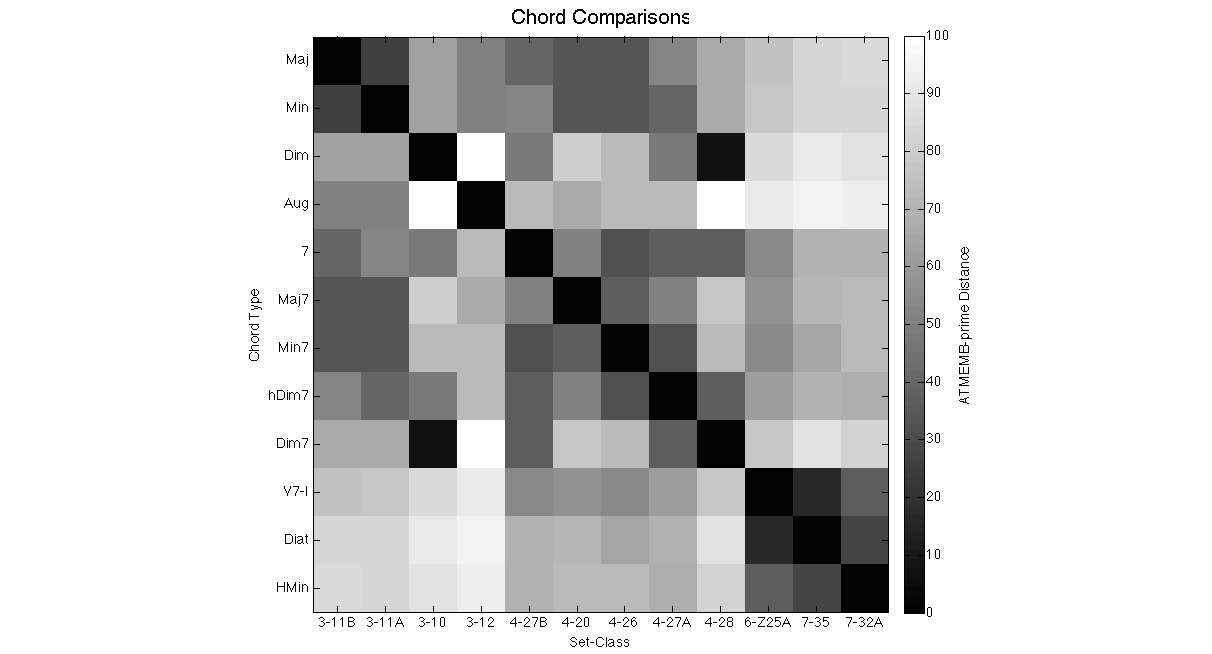
\includegraphics[width=.6\linewidth]{./plots/chordcomp1.png}
\caption{\label{fig:chordcomp1}Chord Comparisons: ATMEMB-prime distances between common tonal objects}
\end{figure}
\begin{figure}[htb]
\centering
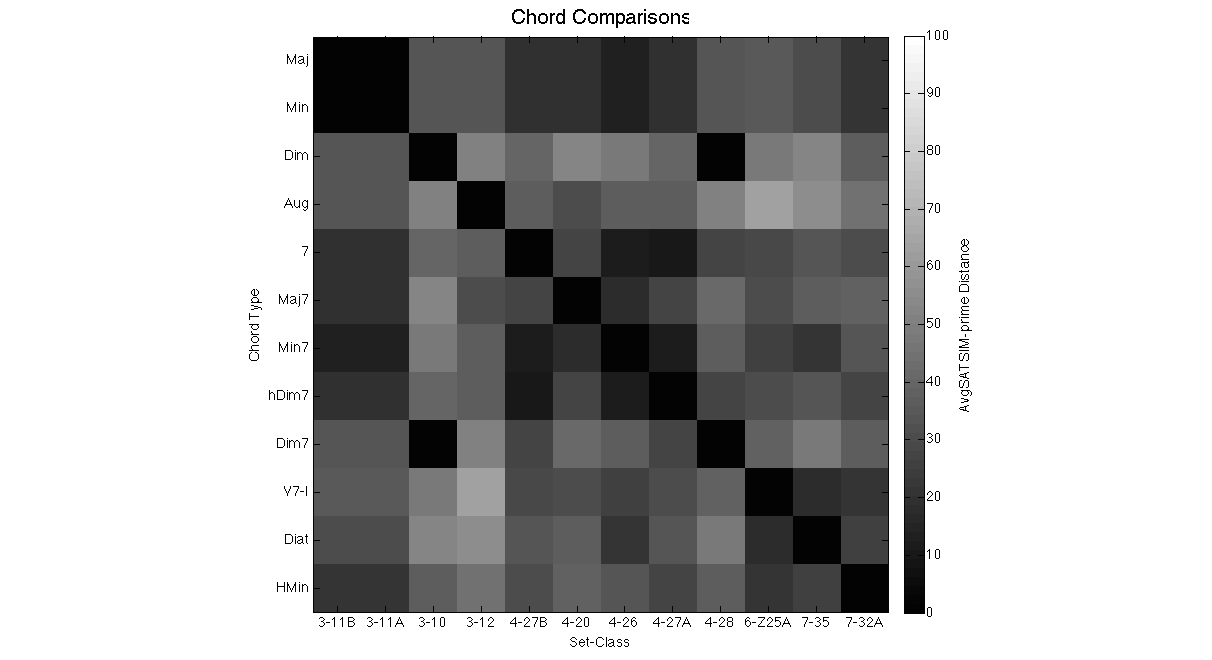
\includegraphics[width=.6\linewidth]{./plots/chordcomp2.png}
\caption{\label{fig:chordcomp2}Chord Comparisons: AvgSATSIM-prime distance between common tonal objects}
\end{figure}

Plotting the absolute difference between the values in these grids
gives a local indication of comparisons for which the measures most
disagree. Figure \ref{fig:measurecomp} shows such a plot, in which the
lighter areas indicate a higher degree of discrepancy between the
measures' values. A more quantitative comparison of the measures can
be obtained by correlation of the vectors containing all 61425
values. Figure \ref{fig:corr} shows a grid with each square
corresponding to a comparison between measures and coloured according
to the correlation value.

\begin{figure}[htb]
 \centering
 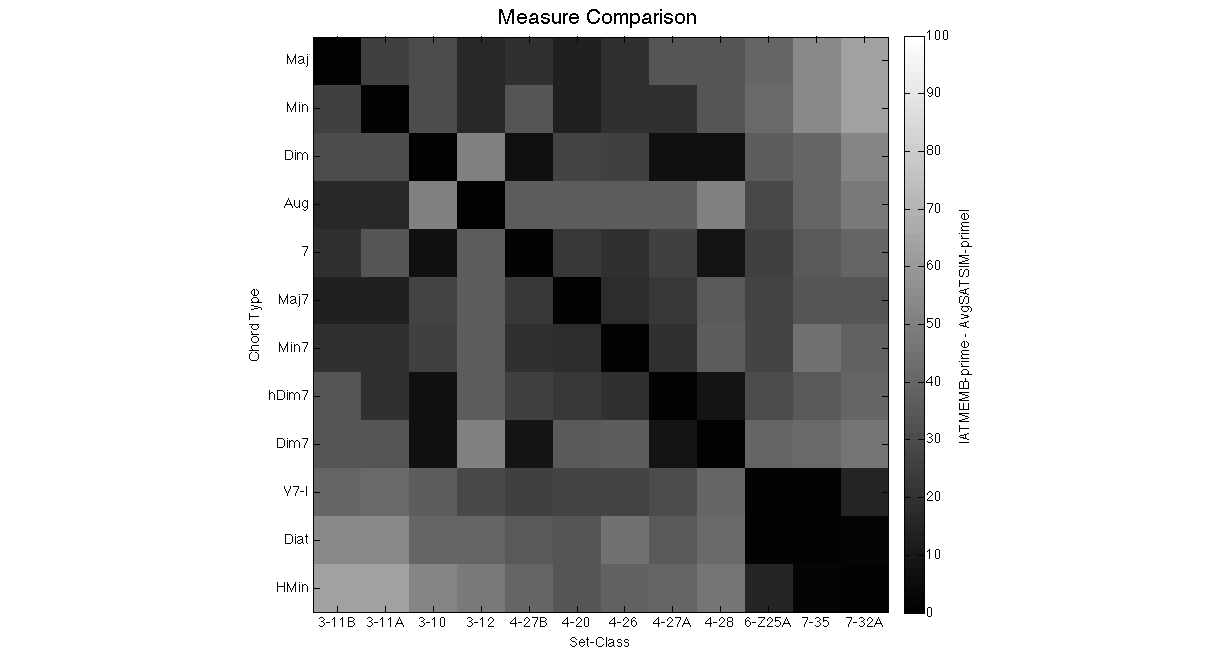
\includegraphics[width=.6\linewidth]{./plots/measurecomp.png}
 \caption{\label{fig:measurecomp}Measure Comparison: Absolute difference between ATMEMB-prime and AvgSATSIM-prime values}
 \end{figure} 
\begin{figure}[htb]
\centering
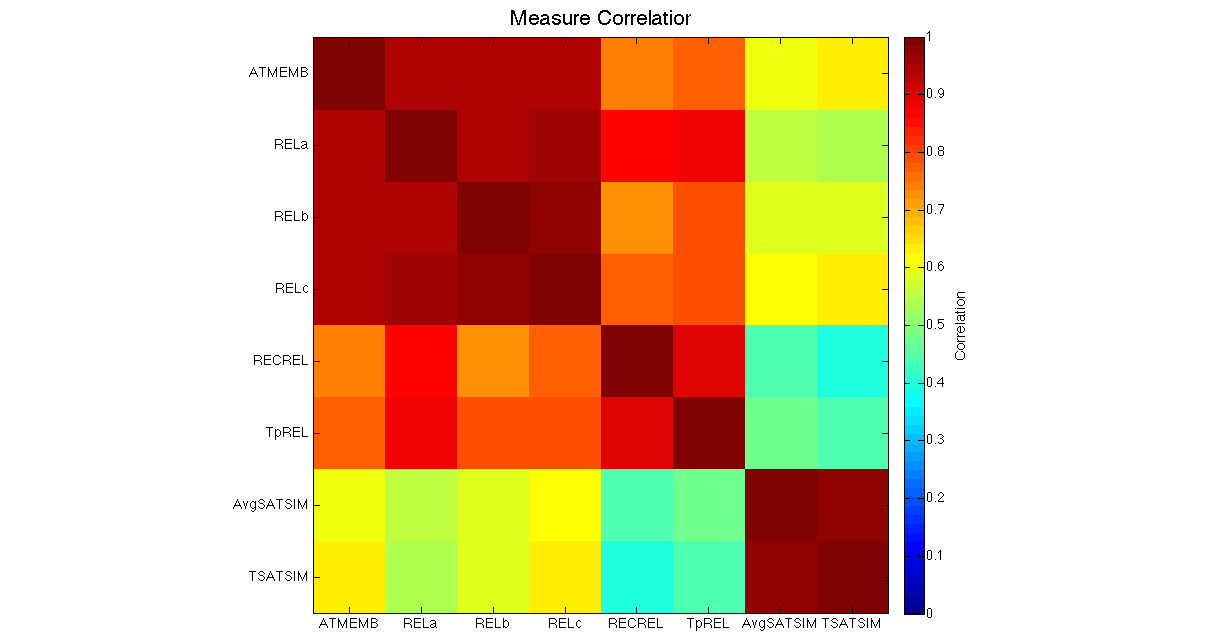
\includegraphics[width=.6\linewidth]{./plots/corr.png}
\caption{\label{fig:corr}Measure Correlation: Correlation between the all the values produced by all measures.}
\end{figure}

The shear quantity of values for all the measures means that a
thorough and meaningful comparison of the would be difficult and time
consuming. Still, from a superficial inspection of these grids it is
possible to draw some basic conclusions:

\begin{enumerate}
\item The values produced by the measures are sufficiently different as to
   produce different outcomes in the proposed analysis.
\item Different measure possess different discriminatory power and give
   different contrast for different collections of set classes.
\item Whilst all the measures can in principle discriminate between
   inversionally related sets only ATMEMB and REL discriminate between
   major and minor triads.
\item AvgSATSIM and TSATSIM are very similar and the values they produce
   are overall lower indicating greater proximity between common chord
   set classes.
\item AvgSATSIM and TSATSIM discriminate poorly between smaller set
   (cardinality 3/4) but between between larger sets (cardinality 7+).
\item The values produced by TPREL are overall higher indicating greater
   separation between common chord set classes.
\item ATMEMB gives a high degree of discrimination between set classes of
   very different cardinalities.
\item RECREL and REL discriminate the best between smaller set classes
   (cardinality 3/4).
\end{enumerate}

\section{Analysis Methodology}
\label{sec-7}

This chapter describes a set of computational techniques that can be used in conjunction
for analysis of a musical piece. \ref{sec-7-1} gives a concise overview of
the analysis process and introduces the key variables whilst \ref{sec-7-2} to \ref{sec-7-4} give a more detailed
explanation of the factors involved in the selection of the
parameters. In the interests of clarity, demonstration of the
techniques with examples will be postponed until chapter \ref{sec-8}.

In this work, analysis is done from digital scores in MIDI format. The
advantage of this is that it avoids the potential inaccuracies
involved in extracting chroma from an audio signal. Symbolic data such
as MIDI allows direct access to the pitch material upon which the
analysis techniques are applied.
\subsection{Overview}
\label{sec-7-1}

The central component in analysis using similarity measures is the
distance time series. This provides a simple means of capturing how
the pitch content of a piece evolves in time with respect to a
specific set class or sonority. It involves segmenting the piece using
a fixed sliding window and calculating the distance between each
segment and a reference set class. Such representations of tonal
progression in time lend themselves very well to analysis of harmonic
and musical structure. Specific features of the curve can indicate
structurally important events while repetitions in the time series can
indicate passages with similar tonal progressions. The first examples
of distance time series are in Figure \ref{fig:refsets} (\ref{sec-8-2}).

There are three interdependent parameters which must be selected
according to the specific intentions of the analyst: Segmentation
(window and hop size), the reference set class and the
similarity/distance measure. The segmentation determines the captured
set class content, which should be targeted according to its
relationship to the reference set class. This relationship is
determined by the measure used, which must possess an adequate degree
of discrimination so as to produce characteristic changes in the time
series.
\subsection{Reference Set Class Selection}
\label{sec-7-2}

Selection of the reference SC will vary depending on the intentions of
the analyst; different selections will reveal different musical
features and types of harmonic structure. In traditional musicology,
the components of harmonic structure are described by scales, chords
and chord progressions. As a preliminary step towards the
reconstruction of this conventional analysis, it is necessary to make
some connections between common musical objects and set class
theory. Appendix \ref{sec-13} contains tables that list common
chords, cadential progressions and scales with their corresponding set
classes. Before selecting a reference set it is necessary to identify
which of these basic groups are most relevant to the analysis aims
i.e. to establish the \texttt{sets of interest}. Below, three potential
reference sets are proposed with and given musicological motivation.

\begin{enumerate}
\item Major/Minor Triad (3-11A/3-11B): The triad is widely considered to
   be the basic building block of western harmony. A distance time
   series with reference to the basic major or minor triad will give
   an indication as to the complexity of the chords and harmonic
   progressions.
\item Perfect Authentic Cadence (6-Z25A): In much of western music
   cadences punctuate harmonic progressions by suggesting varying
   degrees of resolution. A distance time series with reference to the
   perfect authentic cadence might contain characteristic features at
   the boundaries between distinct passages.
\item Diatonic Scale (7-35): The pitch content of much western music is
   confined to the diatonic scale. A distance time series with
   reference to the diatonic set would indicate the degree to which
   the music is diatonic or signal the use of other scales and
   modulations.
\end{enumerate}
\subsection{Segmentation}
\label{sec-7-3}

Using a fixed sliding window to segment the music requires considered
selection of the window length and hop size so as to best target the
\texttt{sets of interest}. The selection of these parameters is a crucial
stage in the analysis process, which is highly sensitive to the scale
of observation. The window size determines the cardinality of the sets
which are captured, with larger windows typically containing larger
cardinality sets. The relationship between hop size and captured set
class contents is rather subtle: smaller hop sizes are required for
observing the note-wise change in set class that occurs in passages of
sequential (horizontal) notes, whereas larger hop sizes can be used
when the harmony is built from concurrent (vertical) notes.

When working in the MIDI domain, an alternative segmentation policy
can be adopted to supplement the analysis process. This method, from
\citet[chap. 5.3]{Martorell2013}, is a fully systematic segmentation
policy which exhaustively windows every possible combination of
adjacent notes. \citet[chap. 5.3.5]{Martorell2013} also specifies two
compact representations of this data as a means of observing the the
global set class content of a piece:
\begin{description}
\item[Class Matrix] is a 2d plot with time on the x axis and set class 
on the y axis. The set class of each window is calculated and plotted 
as a horizontal line.
\item[Class Vector] 
shows the relative active duration of each class in the class-matrix 
expressed as a percentage of the total duration of the piece.
\end{description}

The first examples of class matrix and class vector are shown in
Figure \ref{fig:bach} (\ref{sec-8-1-1}). This information gives a global
indications as to the types of sonorities contained within a piece and
can aid reference set selection. From this complete information it is
also possible to view statistical information about the time scale in
which specific set classes or cardinality classes occur. This
information can inform the selection of window and hop size so as to
best target the sets of interest. The first example of this is in
Figure \ref{fig:bachseg} (\ref{sec-8-1-1}). Once the sliding window
segmentation has been performed, the captured set class contents can
be viewed by superimposing them on top of the class matrix and class
vector. This representation gives an indication of the proportion of
the overall class contents that have been retrieved and thus the
efficacy of the sliding window parameters. The first example of this
is in Figure \ref{fig:BWV-846-red} (\ref{sec-8-3}).
\subsection{Measure Selection}
\label{sec-7-4}

As mentioned previously, different measures may be appropriate for different analysis contexts. Grids
such as those shown in \ref{sec-6-5} form a simple way to
visualise the values produced by a measure and can give an indication
of the relationship between the set classes in a in a specific time
scale. Comparison of these grids can reveal the strengths and
weaknesses of the different measures. Often it is useful to directly
compare the time series produced by two measures by plotting
both. This technique is used throughout \ref{sec-8}. In many
cases this is the simplest way to select the best measure.

A further method available for understanding the relationship between
set classes is through multidimensional scaling. Spaces formed from
the set classes contained in a specific segmentation time scale can be
used for comparing different measures and can aid the selection of
comparison set. Examples of this are in \ref{sec-8-6}.

\section{Analysis Examples}
\label{sec-8}

In this chapter the analytical potential of the similarity measures is
evaluated through specific analysis examples. The subjects of the
analysis are described in \ref{sec-8-1} while, \ref{sec-8-2}
to \ref{sec-8-6} contain examples of the computation techniques
described in \ref{sec-7}.

In examples where distance time series are displayed, different
measures are plotted in different colours. Figure \ref{fig:colourkey}
shows a colour key for these plots. In each example a selection of
measures are presented together for comparison. Each selection is
intended to demonstrate the variation in measure selection.
\begin{figure}[htb]
\centering
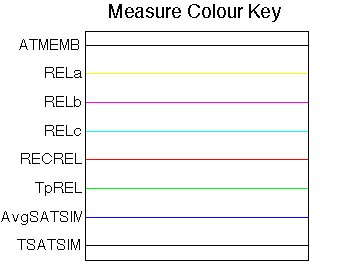
\includegraphics[width=.2\linewidth]{./plots/colourkey.png}
\caption{\label{fig:colourkey}Measure colour key}
\end{figure}
\subsection{Musical Examples}
\label{sec-8-1}

Two pieces were chosen as subjects for analysis:
\begin{enumerate*}[label=\itshape\alph*\upshape)]
\item BWV-846: C Major Prelude from Book I of The Well-Tempered
Clavier by JS Bach
\item Dvorak-Op101-1: Humoresque No. 1, Vivace by Antonín Dvořák.
\end{enumerate*}
Each piece is short and for solo piano/keyboard, which limits the
number of voices complicit in the harmony. In addition, each piece
exemplifies some example of common musical practise.
\subsubsection{BWV-846}
\label{sec-8-1-1}

This piece was chosen for the relative simplicity of its tonal
contents. The harmonic progression is expressed through a series of
arpeggiated chords which are mainly confined to familiar triads and
seventh chords and arranged in common cadential progression. The
structure of the piece is as follows:
\begin{description}
\item[Bars 1-4:] A full cadence in C major
\item[Bars 5-11] Modulation to G major
\item[Bars 12-19] Modulation back to C major
\item[Bars 20-35] Complex extended cadence in C major
\end{description} 
Figure \ref{fig:bach} shows the pianoroll (top), class matrix
(middle) and class vector (bottom) for the prelude. Peaks in the class
matrix correspond to 3-11B (major triads), 4-27B (dominant seventh
chords), 6-Z25A (perfect authentic cadences) and 7-35 (diatonic
scales).  Figure \ref{fig:bachseg} shows the window length
statistics. From these plots it can be see that three and four mainly
occur in windows of around 2 beats.
\begin{figure}[htb]
 \centering
 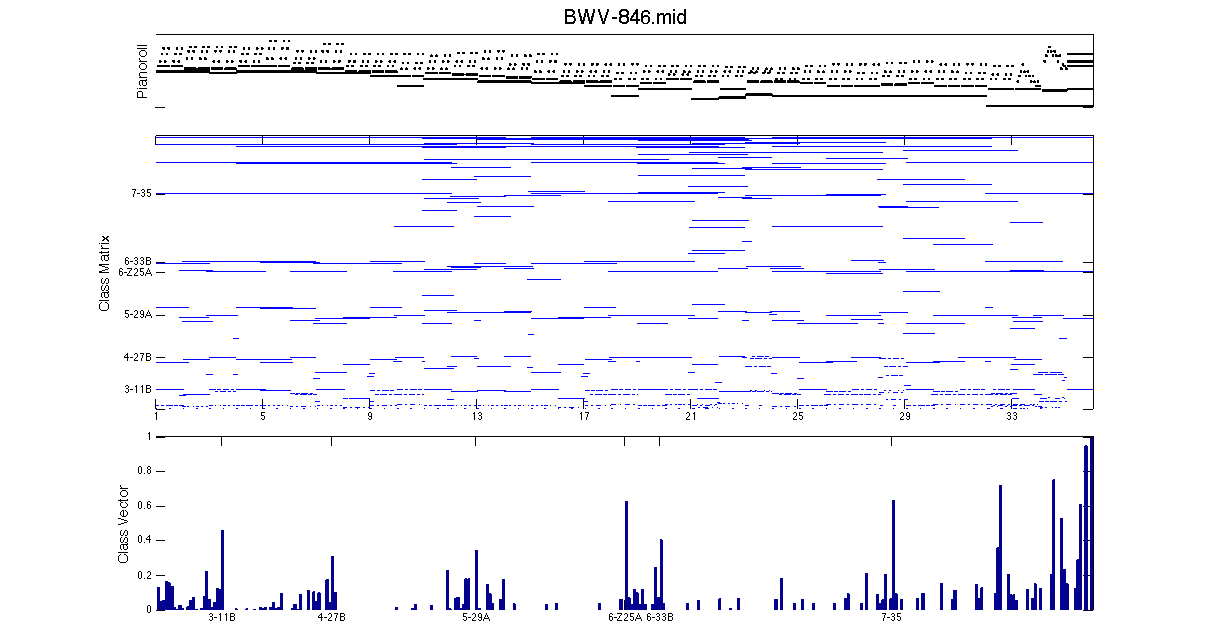
\includegraphics[width=.8\linewidth]{./plots/bach.png}
 \caption{\label{fig:bach}BWV-846: Pianoroll (top), class matrix (middle) and class vector (bottom)}
 \end{figure} 

\begin{figure}[htb]
\centering
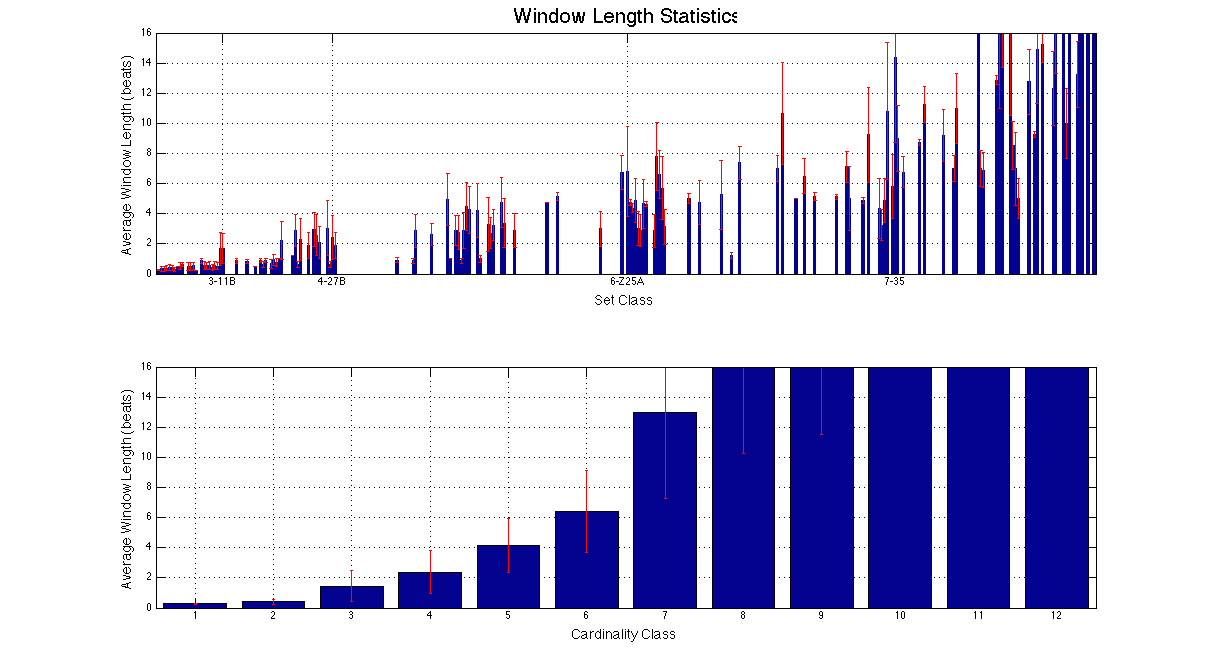
\includegraphics[width=.8\linewidth]{./plots/bachseg.png}
\caption{\label{fig:bachseg}BWV-846: Window length statistics}
\end{figure}
\subsubsection{Dvorak-Op101-1}
\label{sec-8-1-2}

This piece was chosen for its regular structure. It is comprised of
several distinct sections of contrasting tonal material. The piece
starts with the main theme which appears unambiguous in its mode and
tonal centre. This theme is repeated at intervals throughout the
piece. A number of other sections can also clearly be identified. The
sections appear to depart from the tonality of the main theme to
varying degrees. Some sections appear similar to each other save for a
transposition. The identifiable sections of the piece are as follows:
\begin{description}
\item[A] Main theme in Eb (natural) minor
\item[B] Harmonic minor scale (D)
\item[C] Dolce, major mode
\item[D] Stacatto, major mode
\item[C*] Related to C
\item[D*] Related to D
\item[E] Meno Mosso, related to A
\item[F] Finale
\end{description}
Figure \ref{fig:dvorak} shows the pianoroll(top), class matrix
(middle) and class vector (bottom) for the piece. Peaks in the class
matrix correspond to 4-26 (Min7), 5-27B (Min9), 6-32 (Min11), 6-Z25B
(minor cadence) and 7-35. It should be noted that extended chords and
cadences often have the same set class (e.g. Min11 and a $iv-i$
progression). Figure \ref{fig:dvorakseg} shows the window length
statistics for the piece.
\begin{figure}[htb]
\centering
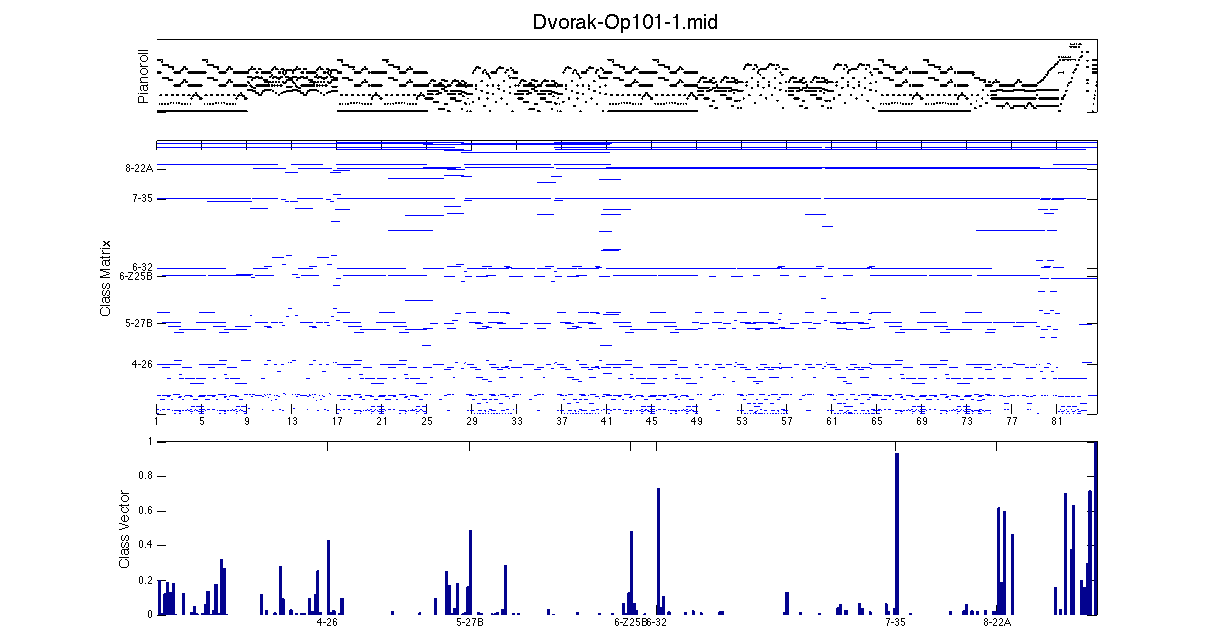
\includegraphics[width=.8\linewidth]{./plots/dvorak.png}
\caption{\label{fig:dvorak}Dvorak-Op101-1: Pianoroll (top), class matrix (middle) and class vector (bottom)}
\end{figure}

\begin{figure}[htb]
\centering
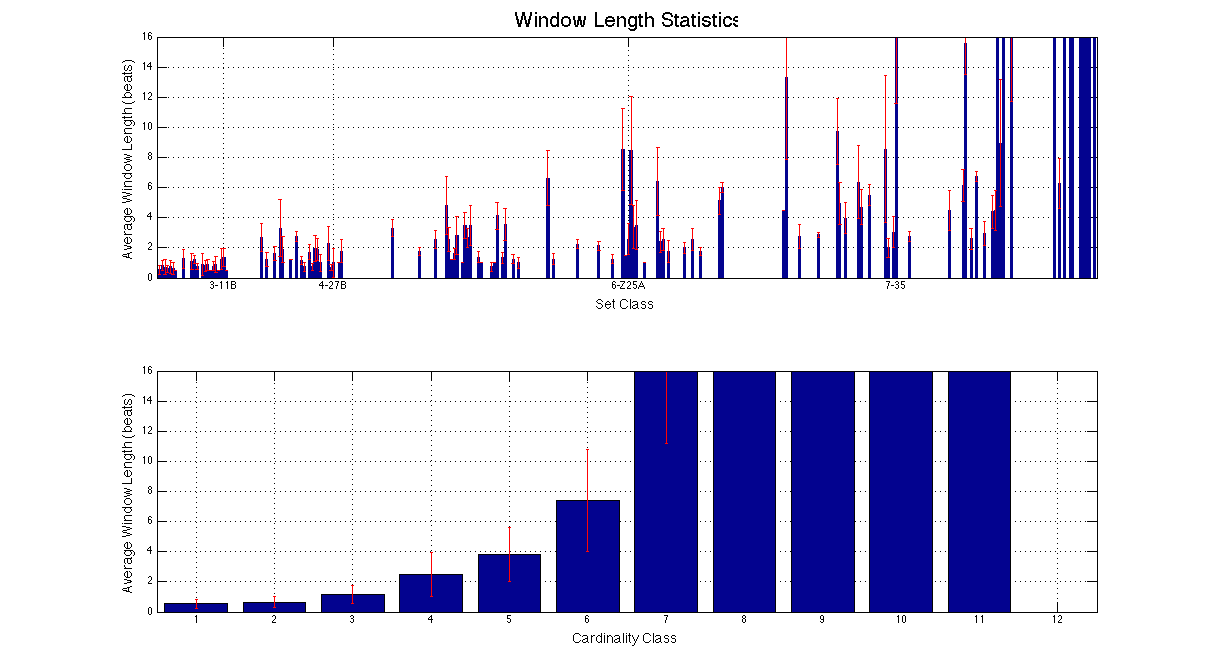
\includegraphics[width=.8\linewidth]{./plots/dvorakseg.png}
\caption{\label{fig:dvorakseg}Dvorak-Op101-1: Window length statistics}
\end{figure}
\subsection{Distance Time Series}
\label{sec-8-2}

\begin{itemize}
\item This example shows how the distance time series can be plotted to
  represent the tonal characteristics of a piece. To facilitate an
  initial, rudimentary analysis example, an reduction of the Bach
  prelude is used (BWV-846-Chords), in which each bar was replaced
  with a single semibreve chord containing every note from that
  bar. This reduction, in effect, replaces the piece with its
  underlying chord progression, removing the rhythmic element of the
  arpeggiation and providing a clearer expression of the tonal
  contents.
\item BWV-846-Chords was segmented using 3 separate sliding windows.
\item Figure \ref{fig:refsets} shows the pianoroll (top) and three
  distance time series, plotted as lines, with reference sets 3-11B,
  6-Z25A and 7-35.
\item 3-11B: Single chords were targeted using a window length of 1 bar
  and a hop size of 1 bar. Thus, each point corresponds to a single
  bar/chord in the progression. Points where the curve is at zero
  correspond to bars containing major triads, while peaks in the curve
  correspond to more complex of less familiar chords.
\item 6-Z25A: Cadential progression were targeted using a window length of
  2 bars and a hop size of 1 bar. Thus, each point corresponds
  adjacent pairs of bars/chords. The occurrence of cadences is marked
  by zeros in the time series.
\item 7-35: Diatonicism was targeted using a window length of 4 bars and a
  hop size of 1 bar. Common in diatonic music of this type are chord
  progressions that move by descending fifths, three of which in
  succession comprise a diatonic set (eg. ii-V-I). Areas of steady
  flatness at zero denote diatonic passages where as the higher points
  in the curve indicate more chromatic passages or less familiar
  scales.
\end{itemize}
\begin{figure}[htb]
\centering
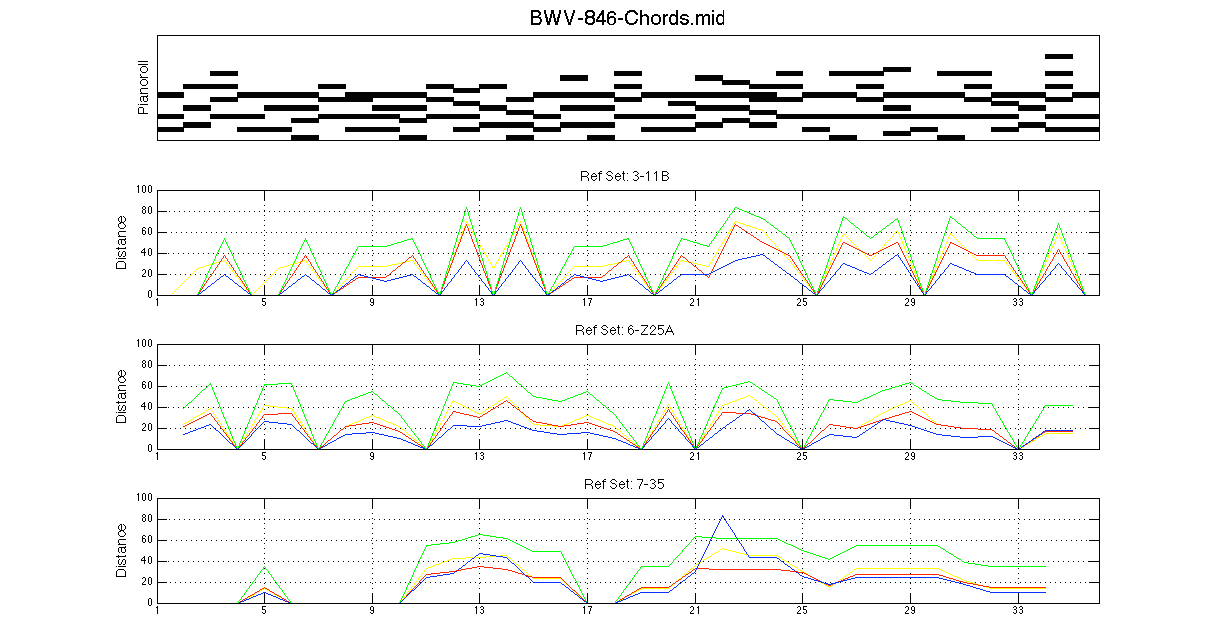
\includegraphics[width=.8\linewidth]{./plots/refsets.png}
\caption{\label{fig:refsets}BWV-846-Chords: Distance time series targeting chords (top), cadences (middle) and diatonicism (bottom).}
\end{figure}
\subsection{Time Series Differential}
\label{sec-8-3}

\begin{itemize}
\item This example shows how the cadential punctuation of a musical piece
  can be detected by calculating the approximate differential of the
  distance time series.
\item BWV-846 was segmented so as to target 3 and 4 note chords using a
  window length of 2 beats. Window size selections was informed by
  Figure \ref{fig:bachseg}. A hop size of 1 beat was chosen so
  as to capture the cadential overlap of these chords.
\item Figure \ref{fig:BWV-846-red} shows the class matrix and class vector
  for BWV-846 with the contents of the sliding superimposed on top in
  red. The class vector shows that a high proportion of major triads
  and seventh chords were captured at this time scale while the class
  matrix shows the position of these captured set classes in time.
\end{itemize}
\begin{figure}[htb]
\centering
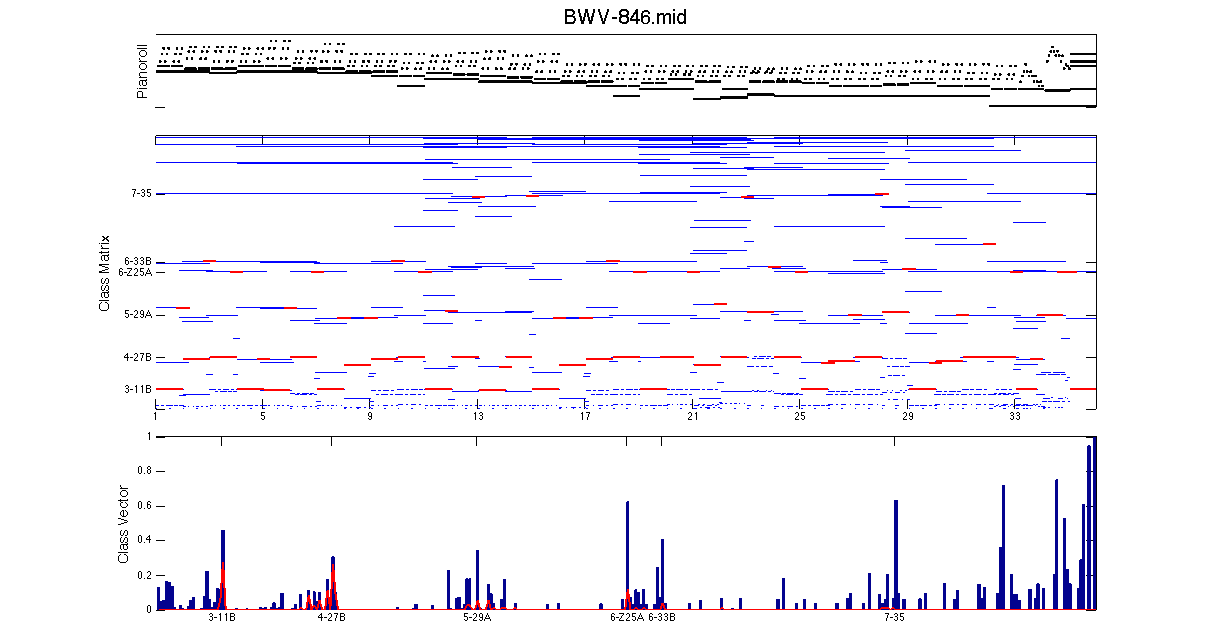
\includegraphics[width=.8\linewidth]{./plots/BWV-846-red.png}
\caption{\label{fig:BWV-846-red}BWV-846: Pinaoroll (top), class matrix (middle) and class vector (bottom) with sliding window contents (red)}
\end{figure}
\begin{itemize}
\item Figure \ref{fig:cadence} shows the pianoroll (top), distance time
  series (middle) and approximate second order differential of the
  time series. The time series was computed using 6-Z25A as a
  reference set.
\item The highest peaks correspond to the centre of windows containing
  perfect authentic cadences ($V^{7}-I$) and denote the boundaries of
  distinct musical units. The first two peaks have been highlighted
  with red arrows and labelled ``A'' and ``B''.
\item The peak at ``A'' in bars 3-4 is at the conclusion of a
  full cadence in C which establishes the tonality of the prelude.
\item The peak at ``B'' in bars 6-7 is where, following a modulation, the
  new key of G major is confirmed with a $V^{7}-I$ cadence.
\end{itemize}
\begin{figure}[htb]
\centering
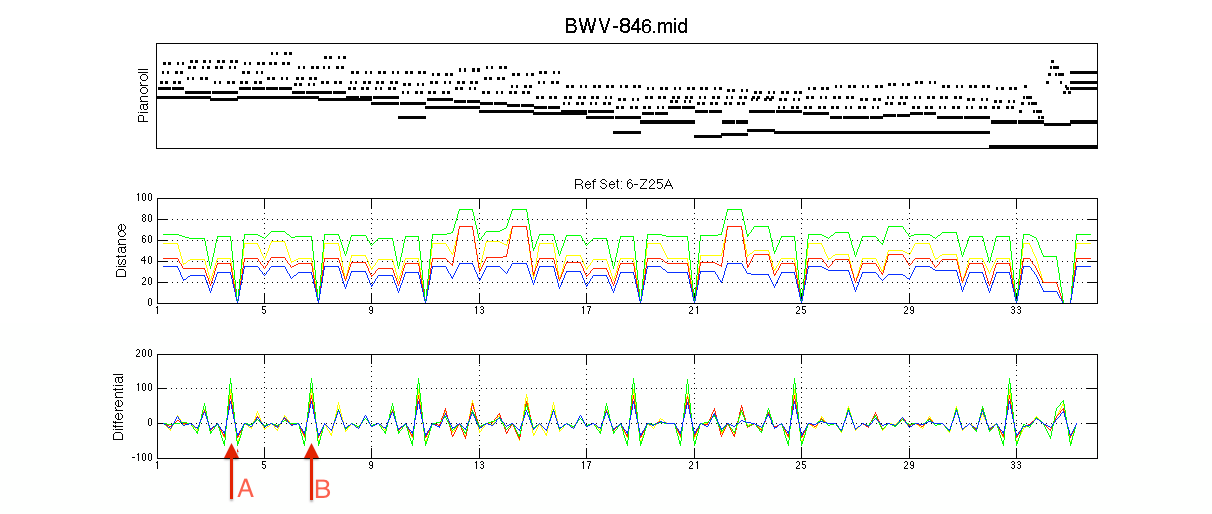
\includegraphics[width=.8\linewidth]{./plots/cadence.png}
\caption{\label{fig:cadence}BWV-846: Cadential punctuation Example 1}
\end{figure}
\begin{itemize}
\item Other types of cadence can be observed by using different comparison
  sets, for example, 7-32B ($vii^{o7}-I$ cadence).
\item A more general approach can involve exploiting the distance between
  subclasses within the cadential classes, such as that between the
  dominant and tonic chords.
\item Figure \ref{fig:cadence2} shows the approximate first order
  differential of the time series computed with reference to 3-11B
  (tonic chord).
\item The negative peaks correspond to sudden drops in the time series
  resulting from the distance between dominant and tonic chords. The
  plot not only marks $V^{7}-I$ cadences but also other types. An example
  has been highlighted with a red arrow and labelled ``C''.
\item The peak marked by ``C'' in bars 14-15 is a $vii^{o7}-I$ cadence as
  part of the modulation back to C major.
\end{itemize}
\begin{figure}[htb]
\centering
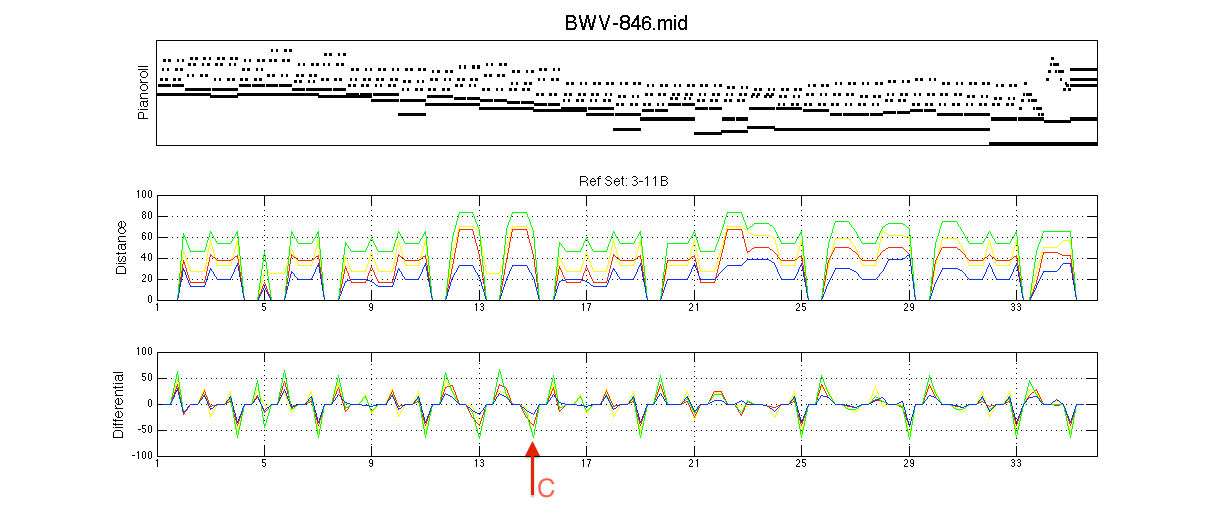
\includegraphics[width=.8\linewidth]{./plots/cadence2.png}
\caption{\label{fig:cadence2}BWV-846: Cadential punctuation Example 2}
\end{figure}
\subsection{Time Series Autocorrelation}
\label{sec-8-4}

\begin{itemize}
\item These examples demonstrates how autocorrelation of the distance time
  series can be used to detect repetitions and some structural aspects
  of the tonal progression.
\item BWV-846 was segmented using a window length of 2 beats and a hop
  size of 1 beat so as to target 3 and 4 note chords.
\item Figure \ref{fig:autocorrelation1} shows the autocorrelation of the
  time series which was calculated using a reference set of
  3-11B. Peaks occur at regular intervals indicating a certain degree
  of structural repetition in the tonal progression. Put another way,
  the time varying distance between the music and 3-11B is periodic,
  repeating at 2 bar intervals.
\end{itemize}
\begin{figure}[htb]
\centering
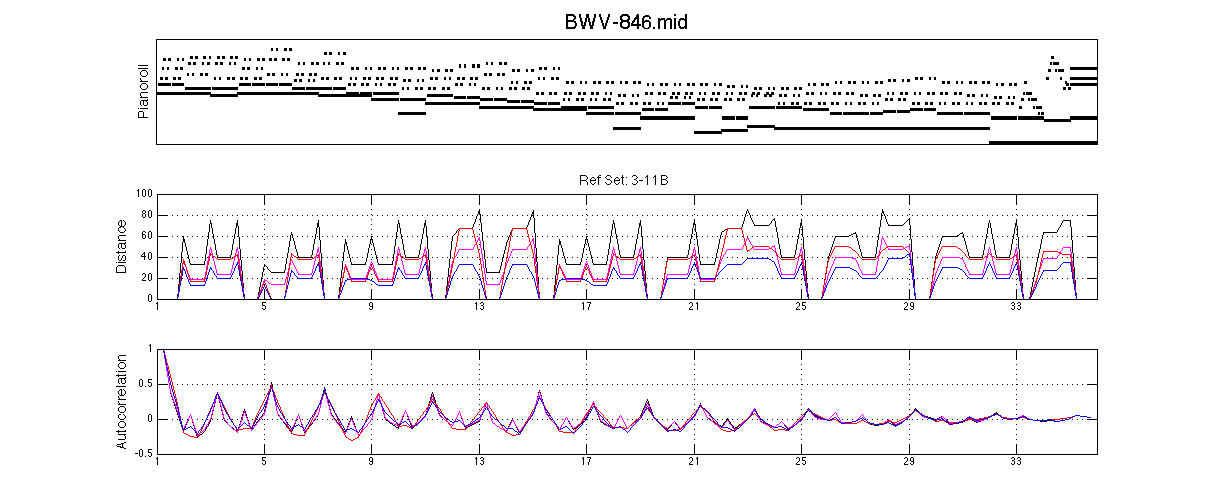
\includegraphics[width=.8\linewidth]{./plots/autocorrelation1.png}
\caption{\label{fig:autocorrelation1}BWV-846: Detection of structural boundaries with autocorrelation}
\end{figure}
\begin{itemize}
\item Dvorak-Op101-1 was segmented so as to target 3 and 4 note chords
  using a window length of 2 beats and hop size of 1 beat. Window
  length selection was informed by figure
  \ref{fig:dvorakseg}.
\item Figure \ref{fig:autocorrelation2} shows the pianoroll (top) with red
  dotted lines marking the boundaries between the structural elements
  of the piece described in \ref{sec-8-1-2}. The distance time series
  (middle) was computed using a reference set of 3-11A. The
  autocorrelation (bottom) shows a similar type of periodicity as
  figure \ref{fig:autocorrelation1} and the pattern of major pattern
  of peaks correspond to the boundaries between section at regular 4
  bar intervals.
\end{itemize}
\begin{figure}[htb]
\centering
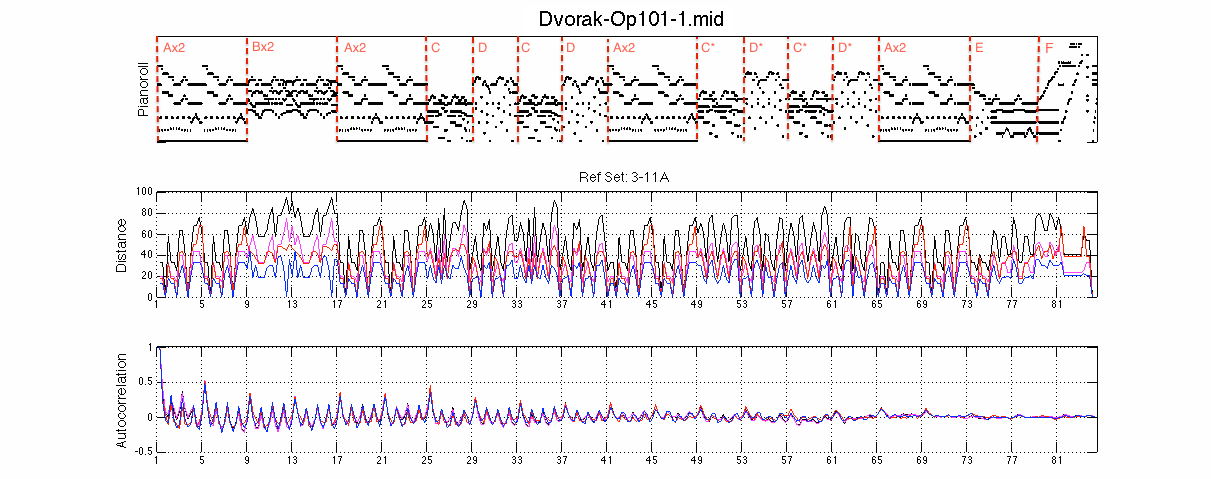
\includegraphics[width=.8\linewidth]{./plots/autocorrelation2.png}
\caption{\label{fig:autocorrelation2}DvorakDvorak-Op101-1: Detection of structural boundaries with autocorrelation}
\end{figure}
\subsection{Self-Similarity Matrix}
\label{sec-8-5}

\begin{itemize}
\item The self-similarity matrix is a widespread technique for detecting
  repetitions in a time series. In this context, the time series is
  the set class time series and the metric used is a set class
  similarity measure.
\item This examples demonstrates how a self-similarity matrix computed in
  this way can be used to obtain structural information about a
  musical piece. Here, there is no need for a reference set as each
  window is systematically compared with every other.
\item Dvorak-Op101-1 was segmented using a window length of 2 beats and
  hop size of 1 beat.
\item Figure \ref{fig:ssm1} shows the self-similarity matrix computed
  using the ATMEMB-prime distance.
\item The area highlighted in red corresponds to section A, the main
  theme, and it can be clearly seen to repeat at various points within
  the piece. The area highlighted in blue shows how the sections C and
  D are related to sections C* and D*. The broken black diagonal down
  the middle of this section indicates the points at which the set
  class material of C* and D* are not identical to C and D.
\end{itemize}
\begin{figure}[htb]
\centering
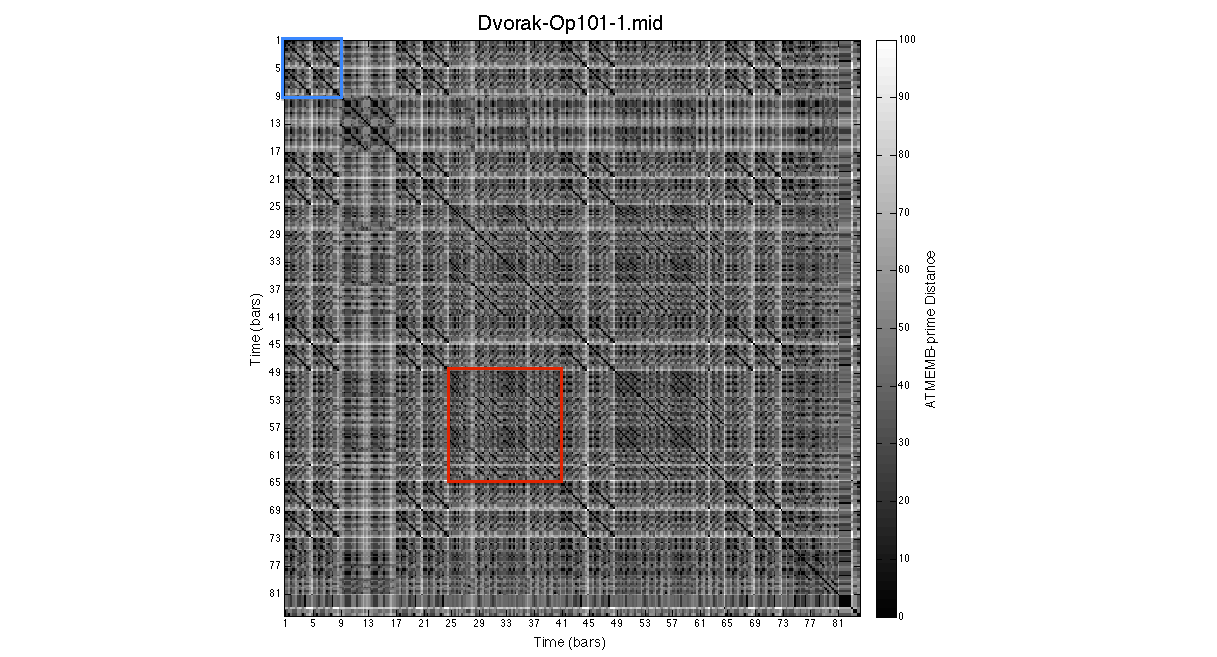
\includegraphics[width=.8\linewidth]{./plots/ssm1a.png}
\caption{\label{fig:ssm1}Dvorak-Op101-1: Self-similarity matrix (ATMEMB-prime)}
\end{figure}
\begin{itemize}
\item BWV-846 was segmented using a window length of 4 beats and hop size
  of 2 beats.
\item Figure \ref{fig:ssm2} shows the self similarity matrix computed
  using the ATMEMB-prime distance.
\item The area highlighted in red contains a black diagonal indicating the
  repetition of a 5 bar sequence: bars 7-11 in G major repeated in
  bars 15-19 in C major. Of additional interest is the region to the
  top left of the area where the diagonal is continued by way of
  several dark grey squares. This shows that there is a small and
  constant distance between these sections, indicating a degree of
  musical similarity that goes beyond mere transposition.
\end{itemize}
\begin{figure}[htb]
\centering
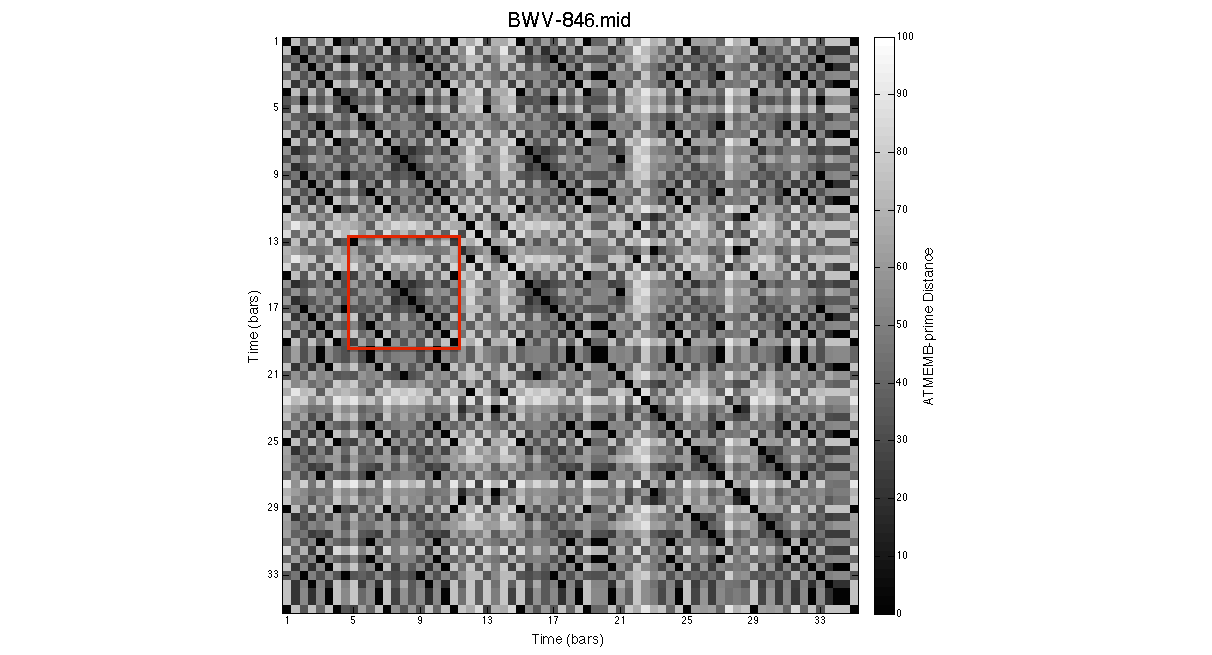
\includegraphics[width=.8\linewidth]{./plots/ssm2.png}
\caption{\label{fig:ssm2}BWV-846: Self-similarity matrix (ATMEMB-prime)}
\end{figure}
\subsection{Set Class Space}
\label{sec-8-6}

\begin{itemize}
\item This example demonstrates how multidimensional scaling can be used to
  visualise a geometric configuration of the set classes captured by a
  specific segmentation policy.
\item Grids such as those shown in \ref{sec-6-5}
\item BWV-486-Chords was segmented with a window length of 1 bar and a hop
  size of 1 bar to obtain the basic chord progression.
\item Figure \ref{fig:1dspace} shows a grid containing the distance values
  between the captured set classes and a reference set of 3-11B. Each
  row contains the values from a different measure and gives a basic,
  1-dimensional projection of the implicit set class space. WHAT DOES
  THIS SHOW?
\end{itemize}
\begin{figure}[htb]
\centering
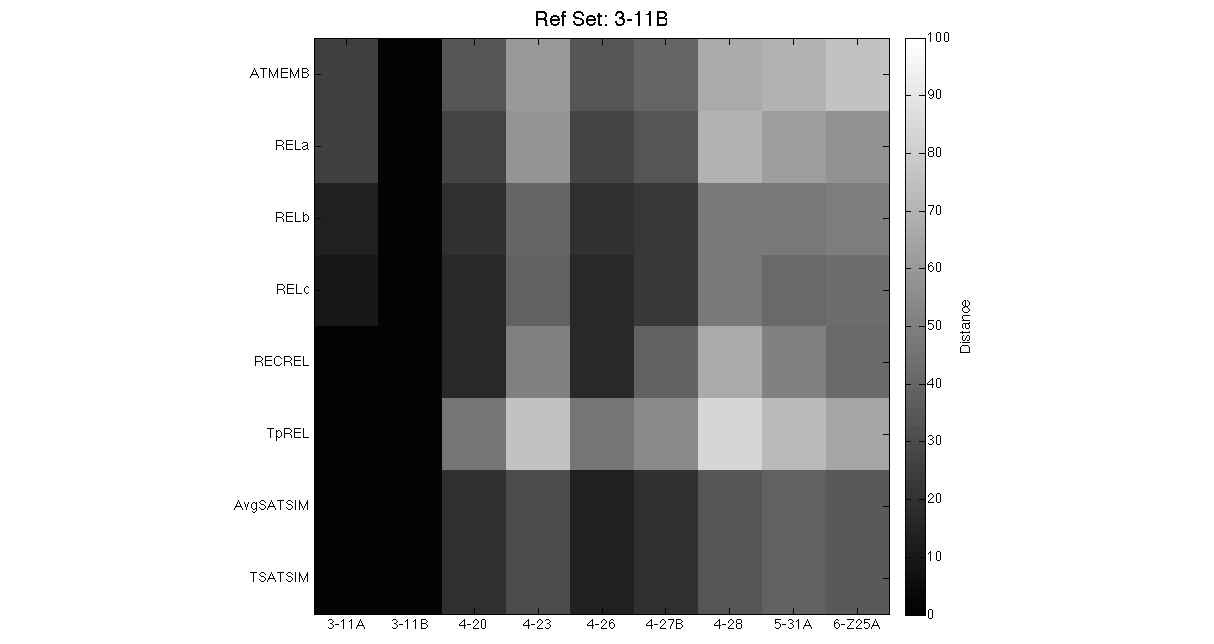
\includegraphics[width=.8\linewidth]{./plots/1dspace.png}
\caption{\label{fig:1dspace}BWV-846-Chords: 1-dimensional set class space}
\end{figure}
\begin{itemize}
\item Figure \ref{fig:scspace1} shows the 2-dimensional configuration
  resulting from non-metric multidimensional scaling of the RELa-prime
  distances between the captured set classes. The size of each point
  is proportional to the relative active duration and they are
  coloured according to a ternary cluster analysis. Although the
  global stress of the configuration is high (0.1967) it gives an
  indication as to the relationship between harmonic components. The
  green cluster contains the chords Maj, Min, 7, Maj7 and Min7 and
  these constitute the greater part of the music. The blue cluster
  contains the perfect cadence and 7sus4 chord which both contain a
  higher number of 4th intervals and occur less frequently. The red
  cluster contains chords Dim7 and Dim7b9 both of which contain high
  numbers of minor 3rds and also occur infrequently.
\end{itemize}
\begin{figure}[htb]
\centering
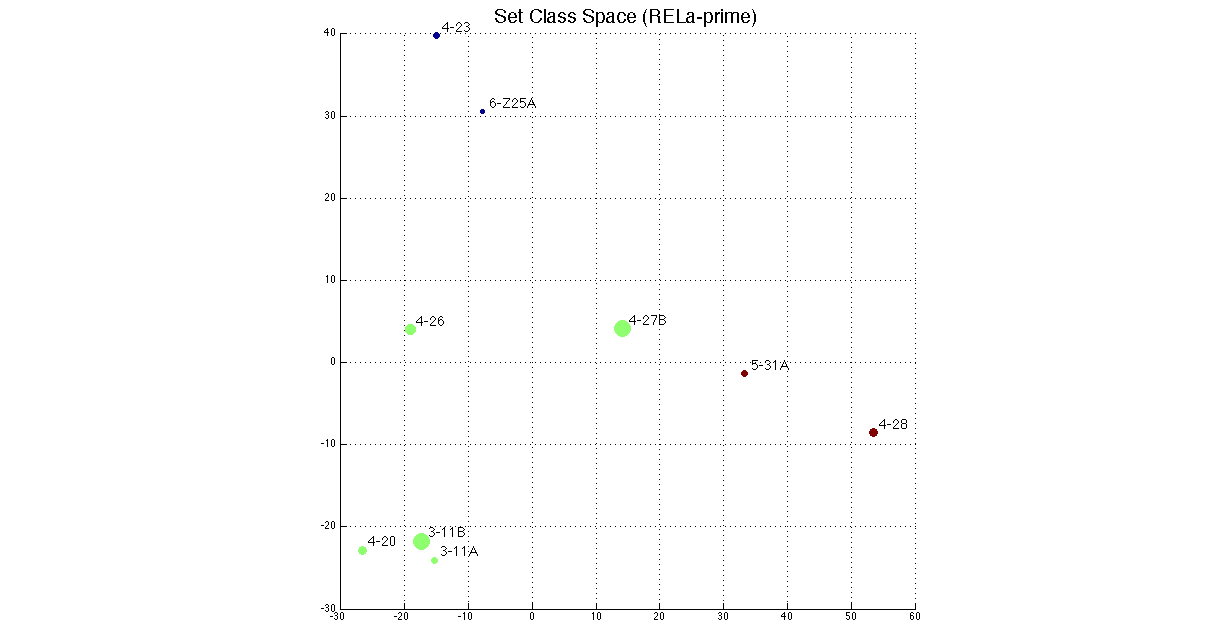
\includegraphics[width=.8\linewidth]{./plots/scspace1.png}
\caption{\label{fig:scspace1}BWV-846-Chords: 2-dimensional chord space (RELa-prime)}
\end{figure}
\begin{itemize}
\item BWV-846-Chords was segmented using a window length of 4 bars and a
  hop size of 1 bar.
\item Figure \ref{fig:scspace2} shows a similar set class space based on
  larger sets (window length of 4 bars and hop size of 1 bar). The
  global stress is 0.0760.
\item The clusters here can be interpreted by the cardinality of the sets
  and amount of chromaticism they contain. A space such as this might
  contain some familiar set classes and others less
  familiar. Visualisation of the space is helpful in understanding the
  material being analysed and could lead to selection of a less
  conventional reference based on its geometric location. A key
  concept to consider when viewing these spaces is that of
  orthogonality. By identifying dimensions that correspond to linearly
  independent properties, the set class space can be better exploited
  in analysis and a better musical and/or mathematical comparison of
  the measures can be performed.
\end{itemize}
\begin{figure}[htb]
\centering
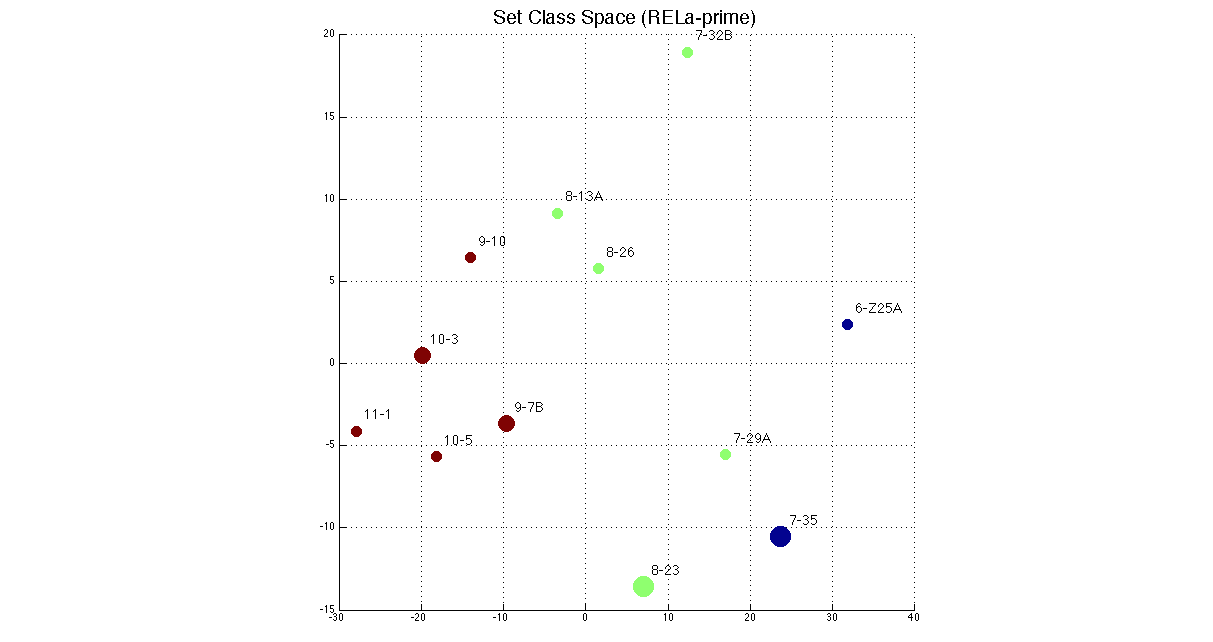
\includegraphics[width=.8\linewidth]{./plots/scspace2.png}
\caption{\label{fig:scspace2}BWV-846-Chords: 2-dimensional scale space (RELa-prime)}
\end{figure}

\clearpage
\part{Discussion}
\section{Conclusions}
\label{sec-9}

\begin{enumerate}
\item This work has successfully demonstrated the analytical potential of
   set class similarity measures.
\item Systematic set class descriptions of music have been discussed in
   terms of their perceptual and analytical relevance and have been
   shown to possess a lot potential as a starting point in many music
   research areas.
\item A comprehensive rendering of musicological concepts and
   terminology in the language of set class theory has facilitated the
   reconstruction of some basic traditional analysis.
\item In isolation, individual sets that correspond to chords of interest
   are of less interest than the hierarchical relationship between
   these sets' subsets and supersets and their evolution in time.
\item A comprehensive survey of set class similarity measures from the
   literature resulted in the selection of six models as suitable
   for systematic descriptive modelling.
\item Basic conclusions were drawn about the different capabilities and
   discriminatory power of the measures, however, it is presumed that
   no one measure is the best: ``There is, after all, no single tool
   makes all other tools obsolete. It is up to each theorist and
   analyst to decide which are appropriate in any given circumstance''
   \citep{Buchler1997}.
\item Two segmentation policies have been presented to work in
   conjunction for extracting a set class description of a musical
   piece: Systematic and sliding window.
\item When working in the symbolic domain, the systematic segmentation
   can be used to supplement the analysis process.
\item The class matrix and class vector are concise and informative
   representations of systematic segmentation data and convey global
   characteristics about a musical piece.
\item The efficacy of a specific sliding window can be assessed by
    plotting the captured contents on top of the class matrix and
    class vector. This technique can be used to tune the window
    parameters so as to target the \texttt{sets of interest}.
\item Five techniques have been presented for representing set class
    information: Distance time series, differential, autocorrelation,
    self-similarity matrix and MDS. These techniques exploit set class
    similarity measures to retrieve structural information.
\item The distance time series has been shown to reflect intuitions about
    the tonal progression of a piece.
\item Approaches to parameter selection can be divided into three
    categories depending on the sets of interest: chords, cadences,
    scales.
\item By targeting common chords and using a reference set of the basic
    triad, the distance time series can be interpreted as reflecting
    harmonic complexity or perhaps musical tension.
\item By targeting two-chord progressions and using a reference set of a
    cadence, the distance time series can characteristic features
    points of cadential punctuation.
\item By targeting scales and using a reference set of the diatonic
    scale, the distance time series can indicate whether the music is
    harmonically stable, very chromatic or modulating.
\item The first and second order differentials of the time series can
    reveal the cadential punctuation of a piece or locate instances of
    any particular set class.
\item Repetitions in the distance time series can be quantified through
    autocorrelation. Peaks in the autocorrelation can point to
    important structural boundaries in a piece.
\item The self-similarity matrix can reveal the structural makeup of a
    piece including repeated sections and related sections.
\item Both autocorrelation and the self-similarity matrix are capable of
    capturing not only exact/transposed repetitions, but passages in
    which some quality of distance or ratio is preserved. These
    relationships are determined by the measure used and might have a
    sophisticated musicological or perceptual basis that is not easily
    observed from listening or from the score.
\item Visualisation of set class space through multi-dimensional scaling
    can give insight into the relationship between tonal objects.
\item Through interpretation of the dimensions, set class spaces can be
    used to understand and compare different measures.
\item Set class spaces constructed using set classes from a specific
    timescale can be used to inform the reference set selection.
\item The large number of interdependent parameters prompted the
    development of an Analysis Tool for MATLAB in which these
    techniques can be used in conjunction, enabling the analyst to
    explore the numerous combinations and approaches. The
    demonstrations here are just the beginning of what could
    potentially be explored.
\item A systematic set class description combined with these
    representation techniques could be employed in MIR systems for the
    automatic detection of structure and musical similarity.
\end{enumerate}

\section{Future Work}
\label{sec-10}

\begin{enumerate}
\item A greater understanding of the set class contents of a piece could
   be achieved through a more exhaustive exploration of systematic set
   class descriptions of simple examples.
\item Understanding the hierarchical relationship between set classes and
   the role of the sets of interest would allow for a more discerning
   selection of parameters.
\item One particularly fascinating line of inquiry is whether the class
   matrix is unique for a given piece. Can pitch classes in the piece
   be changed without changing the class matrix? To what extent can a
   piece be reconstructed from its class matrix?
\item A more concrete and quantitative analysis of the discriminatory
   power of the similarity measures will better inform the selection of
   appropriate comparison sets and measure.
\item A more thorough mathematical evaluation of the measures could be
   starting point for comparison as well as yield information relevant
   to parameter selection.
\item Comparison of set class similarity measures with numerical distance
   measures such as Euclidean and Mahalanobis distance would be a
   necessary component in the justification of their use.
\item Examination of the implicit spaces created by different measures
   could provide an intuitive method of measure
   comparison. Interpretation of the dimensions could reveal the
   musical quantities that they are measuring.
\item Computationally combining different distance plots (multiplying,
   convolving, correlating etc.) could reinforce or weaken a particular
   analytical hypothesis.
\item The addition of peak selecting and structural marking in the
   analysis tool would inform tests as to the suitability of the
   proposed techniques for automatic structual segmentation.
\item The use of multiple measures, comparison sets and sliding windows
    could allow for a more finely tuned targeting of structural
    information.
\item The use of multiple distances simultaneously would allow the
    combining of approaches specified here. It would also be a step
    towards describing tonal progressions in multidimensional space.
\item The use of set class spaces could provide deeper understanding of
    tonal progressions by analogy to trajectories in space.
\end{enumerate}

\clearpage
\bibliographystyle{plainnat}
\bibliography{/Users/nick/Documents/MendeleyDesktop/library.bib}

\clearpage
\part{Appendices}
\appendix
\section{Set Class Similarity Measures}
\label{sec-11}

This chapter contains a concise summary of the set class similarity
measures from the literature organised by theorist. Each section
specifies the publication in which the measure was proposed and brief
description of the theoretical approach adopted by the theorist. A
mathematical formula is given where possible using standard notation. A
reference for notation can be found in \ref{sec-11-1} and commonly used
symbols are defined in the glossary. Where a mathematical formula does
suffice, the comparison procedure is described in words. In addition,
each section contains a table specifying important statistics:
\begin{itemize}
\item SC-Type: the type of SC the measure compares (Tn or TnI)
\item Cardinality: whether the measure can compare SCs of different
  cardinalities.
\item Vector Type: the type of vector used in the comparison procedure
  (see \ref{sec-3-3}).
\item Criteria Met: a list of Castren's criteria which the measure meets.
\item I-related: whether the measure discriminates between inversionally
  related sets.
\item Z-related: whether the measure discriminates between Z-related sets.
\end{itemize}
\subsection{On Notation}
\label{sec-11-1}

Many of the formulas for similarity measures in the following sections
appear differently to the way they were originally published. The
reason for this is an attempt to standardise their symbolic
representation through common vector notation in order to illuminate
and compare the underlying mathematical concepts. Below are
definitions of the of the required symbols.
\begin{description}
\item[Difference Vector] is the absolute
difference between corresponding terms in the nCVs of two SCs, X and Y:\\
$$DV(nCV(X),nCV(Y))=\left|nCV(X)-nCV(Y)\right|$$ \item[Vector
Magnitude] is the length of the nCV in euclidean space:\\
$$\left\|nCV(X)\right\|=\sqrt{\sum_{i=1}^{\#nC}{(nCV(X)_{i})^{2}}}$$
\item[Unit Vector] is the normalised nCV (unit length):\\
$$\hat{nCV(X)}=\frac{nCV(X)}{\left\|nCV(X)\right\|}$$ \item[Euclidean
Distance] is the distance between the points defined by two nCVs in
n-dimensional Euclidean space:\\
$$d(X,Y)=\sqrt{\sum_{i=1}^{n}{(X_{i}-Y_{i})^{2}}}=\left\|DV(X,Y)\right\|$$
\end{description}
\subsection{MORRIS}
\label{sec-11-2}
\subsubsection{K}
\label{sec-11-2-1}

Presented in \citet[pp. 448]{Morris1979}, the K measure gives the
number of intervals-classes (dyad-classes) shared by two SCs, X and Y.
$$ K(X,Y)= \sum_{i=1}^{6}{MIN(x_{i},y_{i})} $$

\begin{center}
\begin{tabular}{ll}
 SC Type:       &  TnI                 \\
 Cardinality:   &  Any                 \\
 Vector Type:   &  ICV                 \\
 Criteria Met:  &  C1,C2,C3.3,C3.4,C4  \\
 I-related:     &  No                  \\
 Z-related:     &  No                  \\
\end{tabular}
\end{center}
\subsubsection{SIM}
\label{sec-11-2-2}

Presented in \citet[pp. 446]{Morris1979}, SIM compares the ICVs of two
SCs (the value is the cardinality of the DV).
$$SIM\left(X,Y\right)=\#DV\left(ICV\left(X\right),ICV\left(Y\right)\right)$$
SIM is also a function of K: $$SIM(X,Y) = \#ICV(X) + \#ICV(Y) -
2.K(X,Y)$$

\begin{center}
\begin{tabular}{ll}
 SC Type:       &  TnI                 \\
 Cardinality:   &  Any                 \\
 Vector Type:   &  ICV                 \\
 Criteria Met:  &  C1,C2,C3.3,C3.4,C4  \\
 I-related:     &  No                  \\
 Z-related:     &  No                  \\
\end{tabular}
\end{center}
\subsubsection{ASIM}
\label{sec-11-2-3}

Presented in \citet[pp. 450]{Morris1979}, ASIM (Absolute SIM) is a
scaled version of SIM to address criteria C3.1. Scaling is done as a
final step. Whilst the scale of values is now fixed, the resolution is
course when cardinalities differ greatly.
$$ASIM\left(X,Y\right)=\frac{SIM\left(X,Y\right)}{\#ICV\left(X\right)+\#ICV\left(Y\right)}$$

\begin{center}
\begin{tabular}{ll}
 SC Type:       &  TnI                      \\
 Cardinality:   &  Any                      \\
 Vector Type:   &  ICV                      \\
 Criteria Met:  &  C1,C2,C3.1,C3.2,C3.4,C4  \\
 I-related:     &  No                       \\
 Z-related:     &  No                       \\
\end{tabular}
\end{center}
\subsection{LORD}
\label{sec-11-3}
\subsubsection{sf}
\label{sec-11-3-1}

Presented in \cite[pp. 93]{Lord1981}, sf (Similarity Function) is
similar to SIM but developed independently. sf is a subset of SIM:
$$sf\left(X,Y\right)=\frac{\#DV\left(ICV\left(X\right),ICV\left(Y\right)\right)}{2}=\frac{SIM(X,Y)}{2}$$

\begin{center}
\begin{tabular}{ll}
 SC Type:       &  TnI           \\
 Cardinality:   &  Same          \\
 Vector Type:   &  ICV           \\
 Criteria Met:  &  C3.3,C3.4,C4  \\
 I-related:     &  No            \\
 Z-related:     &  No            \\
\end{tabular}
\end{center}
\subsection{TEITELBAUM}
\label{sec-11-4}
\subsubsection{s.i.}
\label{sec-11-4-1}

Presented in \citet[pp. 88]{Teitelbaum1965}, s.i. (Similarity Index)
is the Euclidean distance between the Cartesian coordinates defined
by the ICVs of two SCs. This is equivalent to the magnitude of the
difference vector. $$s.i.(X,Y)=\left\|DV(ICV(X),ICV(Y))\right\|$$

\begin{center}
\begin{tabular}{ll}
 SC Type:       &  TnI        \\
 Cardinality:   &  Same       \\
 Vector Type:   &  ICV        \\
 Criteria Met:  &  C3.3,C3.4  \\
 I-related:     &  No         \\
 Z-related:     &  No         \\
\end{tabular}
\end{center}
\subsection{ROGERS}
\label{sec-11-5}
\subsubsection{IcVD$_{1}$}
\label{sec-11-5-1}

Presented in \citet{Rogers1992}, IcVD$_{1}$ (Distance Formula 1) is a
modification of SIM (\ref{sec-11-2-2}). The ICV components are scaled before being
summed. IcVD$_{1}$ is related to Castren's \%REL$_{2}$ (\ref{sec-11-9-3}):
\%REL$_{2}$(X,Y) = IcVD$_{1}$(X,Y)\texttimes{} 50.  

$$IcVD_{1}(X,Y)=\#DV\left(\frac{ICV(X)}{\#ICV(X)},\frac{ICV(Y)}{\#ICV(Y)}\right)$$


\begin{center}
\begin{tabular}{ll}
 SC Type:       &  TnI                      \\
 Cardinality:   &  Any                      \\
 Vector Type:   &  ICV                      \\
 Criteria Met:  &  C1,C2,C3.1,C3.2,C3.4,C4  \\
 I-related:     &  No                       \\
 Z-related:     &  No                       \\
\end{tabular}
\end{center}
\subsubsection{IcVD$_{2}$}
\label{sec-11-5-2}

Presented in \citet{Rogers1992}, IcVD$_{2}$ (Distance Formula 2) is
similar to s.i. (\ref{sec-11-4-1}), but instead returns the Euclidean distance
between the ends of the normalised ICVs.
$$IcVD_{2}(X,Y)=\left\|DV(\hat{ICV(X)},\hat{ICV(Y)})\right\|$$

\begin{center}
\begin{tabular}{ll}
 SC Type:       &  TnI                   \\
 Cardinality:   &  Any                   \\
 Vector Type:   &  ICV                   \\
 Criteria Met:  &  C1,C2,C3.1,C3.2,C3.4  \\
 I-related:     &  No                    \\
 Z-related:     &  No                    \\
\end{tabular}
\end{center}
\subsubsection{Cos($\theta$)}
\label{sec-11-5-3}

Presented in \citet{Rogers1992}, Cos$\theta$, gives the cosine of the
angle between the ICVs in six-dimensional Euclidean space. As the
angle decreases the similarity approaches 1.
$$Cos\theta(X,Y)=\frac{ICV(X)\cdot ICV(Y)}{\left\|ICV(X)\right\|\times\left\|ICV(Y)\right\|}$$

\begin{center}
\begin{tabular}{ll}
 SC Type:       &  TnI                   \\
 Cardinality:   &  Any                   \\
 Vector Type:   &  ICV                   \\
 Criteria Met:  &  C1,C2,C3.1,C3.2,C3.4  \\
 I-related:     &  No                    \\
 Z-related:     &  No                    \\
\end{tabular}
\end{center}
\subsection{RAHN}
\label{sec-11-6}
\subsubsection{AK}
\label{sec-11-6-1}

Presented in \citet[pp. 489]{Rahn1979}, AK is an absolute or adjusted
version of Morris' K (\ref{sec-11-2-1}), addressing the C3.1 criteria. AK is related
to Morris' ASIM: AK(X,Y)=1-ASIM(X,Y).
$$AK\left(X,Y\right)=\frac{2K\left(X,Y\right)}{\#ICV\left(X\right)+\#ICV\left(Y\right)}$$

\begin{center}
\begin{tabular}{ll}
 SC Type:       &  TnI                      \\
 Cardinality:   &  Any                      \\
 Vector Type:   &  ICV                      \\
 Criteria Met:  &  C1,C2,C3.1,C3.2,C3.4,C4  \\
 I-related:     &  No                       \\
 Z-related:     &  No                       \\
\end{tabular}
\end{center}
\subsubsection{MEMB$_{n}$}
\label{sec-11-6-2}

Presented in \citet[pp. 492]{Rahn1979}, MEMB$_{n}$ (Mutual Embedding
Number) compares the nCVs of two SCs for one nC at a time. It measures
the mutual embedding of subsets such that only non-zero components of
the nCVs contribute. By setting n = 2 (MEMB$_{2}$) it compares ICVs.
$$MEMB_{n}\left(X,Y\right)=\sum_{i=1}^{\#nC}{nCV(X)_{i}+nCV(Y)_{i}}$$
such that nCV(X)$_{i}$>0 and nCV(Y)$_{i}$>0. 

\begin{center}
\begin{tabular}{ll}
 SC Type:       &  TnI or Tn           \\
 Cardinality:   &  Any                 \\
 Vector Type:   &  nCV                 \\
 Criteria Met:  &  C1,C2,C3.3,C3.4,C4  \\
 I-related:     &  Yes*                \\
 Z-related:     &  Yes*                \\
\end{tabular}
\end{center}
\subsubsection{TMEMB}
\label{sec-11-6-3}

Presented in \citet[pp. 492]{Rahn1979}, TMEMB (Total Mutual Embedding
Number) counts the mutually embedded subsets of every
cardinality. TMEMB is a total measure.
$$TMEMB\left(X,Y\right)=\sum_{n=2}^{12}MEMB_{n}\left(X,Y\right)$$

\begin{center}
\begin{tabular}{ll}
 SC Type:       &  TnI or Tn         \\
 Cardinality:   &  Any               \\
 Vector Type:   &  nCV               \\
 Criteria Met:  &  C1,C2,C3.3,C4,C5  \\
 I-related:     &  Yes               \\
 Z-related:     &  Yes               \\
\end{tabular}
\end{center}
\subsubsection{ATMEMB}
\label{sec-11-6-4}

Presented in \citet[pp. 494]{Rahn1979}, ATMEMB (Adjusted Total Mutual
Embedding Number) is a scaled version of TMEMB to address criteria
C3.1 (like SIM and ASIM; A and AK). ATMEMB is a total measure.
$$ATMEMB\left(X,Y\right)=\frac{TMEMB\left(X,Y\right)}{2^{\#X}+2^{\#Y}-\left(\#X+\#Y+2\right)}$$

\begin{center}
\begin{tabular}{ll}
 SC Type:       &  TnI or Tn                   \\
 Cardinality:   &  Any                         \\
 Vector Type:   &  nCV                         \\
 Criteria Met:  &  C1,C2,C3.1,C3.2,C3.4,C4,C5  \\
 I-related:     &  Yes                         \\
 Z-related:     &  Yes                         \\
\end{tabular}
\end{center}
\subsection{ISAACSON}
\label{sec-11-7}
\subsubsection{AMEMB2}
\label{sec-11-7-1}

Proposed by \citet[pp. 8]{Isaacson1990}, AMEMB$_{2}$ (Adjusted MEMB$_{2}$)
is a scaled version MEMB$_{2}$ (\ref{sec-11-6-2}), measuring the mutual
embedding of ICs.  $$AMEMB_{2}=\frac{2 \times
MEMB_{2}(X,Y)}{\left(\#X\left(\#X-1\right)+\#Y\left(\#Y-1\right)\right)}$$

\begin{center}
\begin{tabular}{ll}
 SC Type:       &  TnI         \\
 Cardinality:   &  Any         \\
 Vector Type:   &  ICV         \\
 Criteria Met:  &  C1,C2,C3.1  \\
\end{tabular}
\end{center}
\subsubsection{IcVSIM}
\label{sec-11-7-2}

Presented in \citet[pp. 18]{Isaacson1990}, IcVSIM (Interval-Class
Vector Similarity Relation) is the standard deviation of the entries
in the ICVs of two SCs. IcVSIM is a scaled version of
s.i. (\ref{sec-11-4-1}). IdV$_{i}$ is the ith term in the vector defined by
ICV(X)-ICV(Y) and $\overline{DV}$ is the average (mean) of its
entries.
$$IcVSIM(X,Y)=\sqrt{\frac{\sum(IdV_{i}-\overline{IdV})^{2}}{6}}$$

\begin{center}
\begin{tabular}{ll}
 SC Type        &  TnI         \\
 Cardinality:   &  Any         \\
 Vector Type:   &  ICV         \\
 Criteria Met:  &  C1,C2,C3.4  \\
 I-related:     &  No          \\
 Z-related:     &  No          \\
\end{tabular}
\end{center}
\subsubsection{ISIM2}
\label{sec-11-7-3}

Presented in \citet{Isaacson1996}, ISIM2 is a scaled version of IcVSIM
(\ref{sec-11-7-2}). The squre root is taken of each term in the ICVs. Isaacson
argues that each additional instance of an IC contributes less to
similitude. However, \citet{Samplaski2005a} found ISIM2 to be
inconsistent with itself when applying MDS to the values produced.

\begin{center}
\begin{tabular}{ll}
 SC Type        &  TnI         \\
 Cardinality:   &  Any         \\
 Vector Type:   &  ICV         \\
 Criteria Met:  &  C1,C2,C3.4  \\
 I-related:     &  No          \\
 Z-related:     &  No          \\
\end{tabular}
\end{center}
\subsubsection{ANGLE (Isaacson \& Scott)}
\label{sec-11-7-4}

\citet{Scott1998} proposes a geometric method which is identical to
that of Cos/theta (\ref{sec-11-5-3}) but instead gives the size of the
angle in degrees. $$ANGLE(X,Y) = \arccos{Cos\theta(X,Y)}$$

\begin{center}
\begin{tabular}{ll}
 SC Type        &  TnI                   \\
 Cardinality:   &  Any                   \\
 Vector Type:   &  ICV                   \\
 Criteria Met:  &  C1,C2,C3.1,C3.2,C3.4  \\
 I-related:     &  No                    \\
 Z-related:     &  No                    \\
\end{tabular}
\end{center}
\subsection{LEWIN}
\label{sec-11-8}
\subsubsection{REL}
\label{sec-11-8-1}

Presented in \citet{Lewin1979}, REL compares the nCVs of two SCs for
all the nCs. Like MEMB$_{n}$ (\ref{sec-11-6-2}), REL only considers non-zero
entries however, this is achieved by multiplication (taking the
geometric mean) of corresponding nCV terms.

$$REL(X,Y)=\frac{\sum_{i=1}^{p}{\sqrt{SUB(X)_{i}\times SUB(Y)_{i}}}}{\sqrt{\#SUB(X)\times \#SUB(Y)}}$$

where SUB(X) consists of concatenated nCVs and has a length p.

\begin{center}
\begin{tabular}{ll}
 SC Type:       &  TnI or Tn                   \\
 Cardinality:   &  Any                         \\
 Vector Type:   &  nCV                         \\
 Criteria Met:  &  C1,C2,C3.1,C3.2,C3.4,C4,C5  \\
 I-related:     &  Yes                         \\
 Z-related:     &  Yes                         \\
\end{tabular}
\end{center}
\subsubsection{REL$_{2}$}
\label{sec-11-8-2}

\citet{Rahn1979} suggested a number of manifestations of the basic REL
concept including REL$_{2}$ which measures only intervallic similarity.
$$ REL_{2}(X,Y)\frac{2\times\sum\sqrt{(x_{i}y_{i})}}{\sqrt(\#X(\#X-1)\#Y(\#Y-1))} $$

\begin{center}
\begin{tabular}{ll}
 SC Type:       &  TnI                   \\
 Cardinality:   &  Any                   \\
 Vector Type:   &  ICV                   \\
 Criteria Met:  &  C1,C2,C3.1,C3.2,C3.4  \\
 I-related:     &  No                    \\
 Z-related:     &  No                    \\
\end{tabular}
\end{center}
\subsection{CASTREN}
\label{sec-11-9}
\subsubsection{Castrén's Difference Vector}
\label{sec-11-9-1}

Castrén specifies a different type of DV, which we shall call cDV to
distinguish it from the regular DV. It consists of two rows,
$cDV_{x}(X,Y)=X-Y$ and $cDV_{y}(X,Y)=Y-X$. Any negative values in
either of the rows are set to zero.  In addition Castren defines the
weighted difference vector (wcDV) of two vectors X and Y as:
$$wcDV=\frac{cDV(X,Y)}{\#cDV(X,Y)}\times 100$$
\subsubsection{nC\%V}
\label{sec-11-9-2}

Presented in \citet{Castren1994} for use in \%REL$_{n}$, nC\%V(X) (n-class
subset percentage vector) gives the percentage subset-class contents
of an SC, X. The 2C\%V is the Interval percentage vector.
$$nC\%V(X)_{i}=\frac{nCV(X)_{i}}{\#nCV(X)}\times 100$$
\subsubsection{\%REL$_{n}$}
\label{sec-11-9-3}

Presented in \citet{Castren1994}, \%REL$_{n}$ (Percentage Relation) is a
modification of sf (\ref{sec-11-3-1}) using the nC\%Vs (\ref{sec-11-9-2}) instead of
ICVs. \%REL$_{n}$ can be used as a stand-alone measure, however it is
primarily intended as an intermediate step in T\%REL and RECREL (\ref{sec-11-9-4}
and \ref{sec-11-9-5}). $$\%REL_n(X,Y)=\frac{\#DV(nC\%V(X),nC\%V(Y))}{2}$$

\begin{center}
\begin{tabular}{ll}
 SC Type        &  TnI or Tn                     \\
 Cardinality:   &  Any                           \\
 Measure Type:  &  Single nC                     \\
 Vector Type:   &  nC\%V                         \\
 Criteria Met:  &  C1,C2,C3.1,C3.2,C3.3,C3.4,C4  \\
 I-related:     &  Sometimes                     \\
 Z-related:     &  Sometimes                     \\
\end{tabular}
\end{center}
\subsubsection{T\%REL}
\label{sec-11-9-4}

Presented in \citet{Castren1994}, T\%REL (Total Percentage Relation) is
the mean average of the values of \%REL$_{n}$ for all values of $n$ from
$2$ to $m$ where, if $\#X\neq\#Y$, $m = MIN(\#X,\#Y)$ else $m=\#X-1$.
$$T\%REL(X,Y)=\frac{\sum_{n=2}^{m}{\%REL_n\left(X,Y\right)}}{m-1}$$

\begin{center}
\begin{tabular}{ll}
 SC Type:       &  TnI or Tn                        \\
 Cardinality:   &  Any                              \\
 Measure Type:  &  Total                            \\
 Vector Type:   &  nC\%V                            \\
 Criteria Met:  &  C1,C2,C3.1,C3.2,C3.3,C3.4,C4,C5  \\
 I-related:     &  Yes                              \\
 Z-related:     &  Yes                              \\
\end{tabular}
\end{center}
\subsubsection{RECREL}
\label{sec-11-9-5}

Presented in \citet{Castren1994}, RECREL (Recursive Relation)
recursively compares the subsets and subsets of subsets of two SCs
using \%REL$_{n}$ (\ref{sec-11-9-3}). The comparison procedure is quite
complicated and potentially involves evaluating \%REL$_{n}$ thousands of
times. The full algorithm is explained in \citet[]{Castren1994}.

\begin{center}
\begin{tabular}{ll}
 SC Type:       &  TnI or Tn  \\
 Cardinality:   &  Any        \\
 Measure Type:  &  Total      \\
 Vector Type:   &  nC\%V      \\
 Criteria Met:  &  All        \\
 I-related:     &  Yes        \\
 Z-related:     &  Yes        \\
\end{tabular}
\end{center}
\subsection{BUCHLER}
\label{sec-11-10}
\subsubsection{nSATV}
\label{sec-11-10-1}

Presented in \citet[chap. 2.3]{Buchler1997} nSATV(X) (Saturation
Vector) is a dual vector consisting of two rows, nSATV$_{A}$(X) and
nSATV$_{B}$(X). It shows extent to which an SC is saturated with
subclasses of cardinality n. The steps for computing nSATV(X) are
as follows:

\begin{enumerate}
\item Compute the nCVs for all SCs of cardinality \#X.
\item Find the minimum and maximum values for each vector position. These
   values form vectors $Max_{n}(\#X)$ and $Min_{n}(\#X)$.
\item Compute the following two vectors:
   $MaxMinus=DV(nCV(X),Max_{n}(\#X))$ and $MinPlus=DV(nCV(X),Min_{n}(\#X))$
\item $nSATV_{A}(X)_{i}=MIN(MaxMinus_{i},MinPlus_{i})$ and
   $nSATV_{B}(X)_{i}=MAX(MaxMinus_{i},MinPlus_{i})$
\item If $MaxMinus_{i}=MinPlus_{i}$, $nSATV_{A}(X)_{i}=MaxMinus_{i}$
   and $nSATV_{B}(X)_{i}=MinPlus_{i}$
\end{enumerate}
\subsubsection{SATSIM$_{n}$}
\label{sec-11-10-2}

Presented in \citet[chap. 2.4]{Buchler1997}, SATSIM$_{n}$ (Saturation
Similarity index) compares the nSATVs of two SCs and involves the
following steps:
\begin{enumerate}
\item Calculate nSATV(X) and nSATV(Y)
\item Calculate the vectors nSATV$_{\mathrm{row}}$(X) and nSATV$_{\mathrm{row}}$(Y).
\item The function ``row'' maps the MaxMinus values of one nSATV to the
   MaxMinus values of the other. If nSATV$_{A}$(X)$_{i}$ is a MaxMinus
   value and nSATV$_{A}$(X)$_{i}$ is also a MaxMinus value, row = A
   (nSATV$_{\mathrm{row}}$(X)$_{i}$ = nSATV$_{A}$(X)$_{i}$), otherwise row = B.
\item Finally SATSIM$_{n}$(X,Y) is given by the formula:
\end{enumerate}

$$SATSIM_{n}(X,Y)=\frac{\#DV(nSATV_{A}(X),nSATV_{row}(Y))+\#DV(nSATV_{A}(Y),SATV_{row}(X))}{\#DV(nSATV_{A}(X),SATV_{B}(X))+\#DV(SATV_{A}(Y),SATV_{B}(Y))}$$

\begin{center}
\begin{tabular}{ll}
 SC Type:       &  TnI or Tn   \\
 Cardinality:   &  Any         \\
 Measure Type:  &  nC          \\
 Vector Type:   &  nSATV       \\
 Criteria Met:  &  C1,C2,C3.1  \\
 I-related:     &  Sometime    \\
 Z-related:     &  Sometime    \\
\end{tabular}
\end{center}
\subsubsection{AvgSATSIM}
\label{sec-11-10-3}

Presented in \citet[chap. 2.10]{Buchler1997}, AvgSATSIM (Average
Saturation Similarity index) is the mean of SATSIM$_{n}$ values where
$m=MIN(\#X,\#Y)$. $$AvgSATSIM(X,Y)=\frac{\sum_{n=2}^{m-1}{SATSIM_{n}(X,Y)}}{m-2}$$

\begin{center}
\begin{tabular}{ll}
 SC Type:       &  TnI or Tn      \\
 Cardinality:   &  Any            \\
 Measure Type:  &  TOTAL          \\
 Vector Type:   &  nSATV          \\
 Criteria Met:  &  C1,C2,C3.1,C5  \\
 I-related:     &  Yes            \\
 Z-related:     &  Yes            \\
\end{tabular}
\end{center}
\subsubsection{TSATSIM}
\label{sec-11-10-4}

Presented in \citet[chap. 2.10]{Buchler1997}, TSATSIM (Total
Saturation Vector Similarity index) is an extension of
SATSIM$_{n}$. TSATSIM is the quotient of the sum of all SATSIM$_{n}$
numerators and denominators for all values of n from 2 to m-1 where
$m=MIN(\#X,\#Y)$.

\begin{center}
\begin{tabular}{ll}
 SC Type:       &  TnI or Tn      \\
 Cardinality:   &  Any            \\
 Measure Type:  &  TOTAL          \\
 Vector Type:   &  nSATV          \\
 Criteria Met:  &  C1,C2,C3.1,C5  \\
 I-related:     &  Yes            \\
 Z-related:     &  Yes            \\
\end{tabular}
\end{center}
\section{Total Measures: Additional Information}
\label{sec-12}

This appendix contains information regarding the specific formulation
of the total measure, in particular, how they deal with comparisons
involving the trivial forms.
\subsection{Trivial Forms}
\label{sec-12-1}

Three of the 351 Tn-type SCs are known as trivial forms: 1-1, 11-1 and
12-1. Due to their lack of musical or harmonic significance, these SCs
are usually excluded from the work of SC-theorists. However, it is
important that they be included in any systematic description and that
their similarity to other sets be given a meaningful value.

The total measures make comparisons based on the subset content of a
set. SC 1-1, which has no subsets, is rarely accounted for in such
measures and in these cases a simple method will be used: Comparisons
involving X = 1-1 and Y will be given the value $1\#Y$. Thus, the
value will be the ratios of the cardinalities with 1 indicating
maximum similarity.
\begin{table}[htb]
\caption{Trivial Forms} 
\begin{center}
\begin{tabular}{rl}
  1-1  &  \{0\}                          \\
 11-1  &  \{0,1,2,3,4,5,6,7,8,9,10\}     \\
 12-1  &  \{0,1,2,3,4,5,6,7,8,9,10,11\}  \\
\end{tabular}
\end{center}
\end{table}
\subsection{Scale of Values}
\label{sec-12-2}

The values of each measure were adjusted to the same scale for
comparability by the same method as \citet[pp. 48]{Kuusi2001}). This
scale is from 0 to 100 with with 0 indicating maximum similarity. The
modified values are signalled by adding the symbol ``prime'' to the
name.
\begin{table}[htb]
\caption{Adjustment for MEASURE-prime scale} 
\begin{center}
\begin{tabular}{lll}
 ATMEMB-prime(X,Y)     &  $=$  &  (1-ATMEMB(X,Y))*100  \\
 REL-prime(X,Y)        &  $=$  &  (1-REL(X,Y))*100     \\
 AvgSATSIM-prime(X,Y)  &  $=$  &  T\%REL(X,Y)          \\
 TSATSIM-prime(X,Y)    &  $=$  &  RECREL(X,Y)          \\
 TpREL-prime(X,Y)      &  $=$  &  AvgSATSIM(X,Y)*100   \\
 RECREL-prime(X,Y)     &  $=$  &  TSATSIM(X,Y)*100     \\
\end{tabular}
\end{center}
\end{table}
\subsection{ATMEMB (Rahn)}
\label{sec-12-3}

Details on how to calculate ATMEMB are give in \ref{sec-11-6-4}. In his analysis
of the measure, Castren concludes that ``divisor term is flawed,
resulting in values suggesting suspiciously high degrees of
dissimilarity between SCs of clearly different cardinalities. The
general reliability and usefulness of the measure is difficulty to
determine'' \citep[pp. 89]{Castren1994}. The trivial forms 11-1 and
12-1 are accommodated explicitly by the formulation of
\citet{Rahn1979}, however SC 1-1 is not and thus values will be
obtained using the method specified in \ref{sec-12-1}.
\subsection{REL (Lewin)}
\label{sec-12-4}

Details on how to calculate REL are given in \ref{sec-11-8-1}. From the basic
equation it is possible to define three different formulations
depending on the exact nature of SUB(X). In each formulation the
trivial forms 11-1 and 12-1 are accommodated. The three formulations
are as follows:
\begin{enumerate}
\item SUB(X) consists of the concatenated nCVs from 2 to 12. Here
   comparisons involving SC 1-1 will be evaluated with the method
   specified in \ref{sec-12-1}.
\item SUB(X) consists of the concatenated nCVs from 1 to 12 (\$1CV(X) =
   \#X\%). This formulation accommodates SC 1-1.
\item \citet{Martorell2013} specifies an alternative formulation where
   SUB(X) begins with the ICV (2CV) followed by the concatenated nCVs
   from 1 to 12. This formulation accommodates SC 1-1.
\end{enumerate}
\subsection{AvgSATSIM and TSATSIM (Buchler)}
\label{sec-12-5}

Details on how to calculate AvgSATSIM and TSATSIM are given in
\ref{sec-11-10-3} and \ref{sec-11-10-4} respectively. Comparisons involving SC 1-1 are
not accommodated and thus the method specified in \ref{sec-12-1} will
be used to provide values. Comparisons involving SCs 11-1 and 12-1 are
accommodated except for the single comparison that involves both. This
is because their MAX$_{n}$(\#X) and MIN$_{n}$(\#X) vectors are equal and
thus all terms of the nSATVs are 0. The value for this comparison will
be set to 0 (indicating maximal similarity). For comparisons involving
ICs the value will be given by SATSIM$_{2}$(X,Y) (see \ref{sec-11-10-2}).
\subsection{T\%REL and RECREL (Castren)}
\label{sec-12-6}

Details on how to calculate T\%REL and RECREL are given in \ref{sec-11-9-4} and
\ref{sec-11-9-5} respectively. Comparisons involving SCs 11-1 and 12-1 are
accommodated in both by Castren's formulation. Comparisons involving
SC 1-1 will be given values by the method specified in \ref{sec-12-1}. Castren comments that some T\%REL values are too high to be
intuitively plausible. Finally, it should be noted that the basic
algorithm provided by Castren for calculating RECREL is not feasible
for large sets. Comparisons of such sets require tables of pre-computed
branch values.
\section{Set Class Reference}
\label{sec-13}

This appendix contains a reference guide for converting common
musicological terminology into the language of set class theory. Table
\ref{tab:chords} contains common chord types and their corresponding
set classes. Table \ref{tab:scales} contains common scales and their
corresponding set classes. Both tables also include the Forte Name and
the Tn-type index of the set classes. Table \ref{tab:cadences}
contains common chord pairs and cadential progression. Each position
in the table contains the set class composed of the two chords
corresponding to the row and the column. Chord symbols are in standard
roman numeral notation.
\begin{table}[htb]
\caption{Chords to set classes} \label{tab:chords}
\begin{center}
\begin{tabular}{lllr}
\hline
 Chord           &  Set Class           &  Name    &  Idx  \\
\hline
 Maj             &  \{0,4,7\}           &  3-11B   &   25  \\
 Maj7            &  \{0,1,5,8\}         &  4-20    &   57  \\
 Maj9            &  \{0,1,3,5,8\}       &  5-27A   &  116  \\
 Maj11           &  \{0,1,3,5,6,8\}     &  6-Z25A  &  176  \\
 Maj13           &  \{0,1,3,5,6,8,10\}  &  7-35    &  276  \\
 Maj(6)          &  \{0,3,5,8\}         &  4-26    &   64  \\
 Maj(6/9)        &  \{0,2,4,7,9\}       &  5-35    &  130  \\
\hline
 7               &  \{0,3,6,8\}         &  4-27B   &   66  \\
 9               &  \{0,2,4,6,9\}       &  5-34    &  129  \\
 11              &  \{0,2,4,6,7,9\}     &  6-33B   &  189  \\
 13              &  \{0,1,3,5,6,8,10\}  &  7-35    &  276  \\
 7b9             &  \{0,2,3,6,9\}       &  5-31B   &  125  \\
\hline
 min             &  \{0,3,7\}           &  3-11A   &   24  \\
 min7            &  \{0,3,5,8\}         &  4-26    &   64  \\
 min9            &  \{0,3,5,7,8\}       &  5-27B   &  117  \\
 min11           &  \{0,2,4,5,7,9\}     &  6-32    &  187  \\
 min13           &  \{0,1,3,5,6,8,10\}  &  7-35    &  276  \\
 min(6)          &  \{0,2,5,8\}         &  4-27A   &   65  \\
 min(b6)         &  \{0,1,5,8\}         &  4-20    &   57  \\
 min(6/9)        &  \{0,2,5,7,8\}       &  5-29B   &  121  \\
 min7b9          &  \{0,3,5,6,8\}       &  5-23B   &  113  \\
\hline
 min/Maj7        &  \{0,1,4,8\}         &  4-19A   &   55  \\
 min/Maj9        &  \{0,1,3,4,8\}       &  5-Z17   &   98  \\
 min/Maj11       &  \{0,1,3,4,6,8\}     &  6-Z24B  &  174  \\
 min/Maj13       &  \{0,1,3,4,6,8,10\}  &  7-34    &  275  \\
\hline
 Dim             &  \{0,3,6\}           &  3-10    &   23  \\
 hDim7           &  \{0,2,5,8\}         &  4-27A   &   65  \\
 hDim7(9)        &  \{0,2,4,5,8\}       &  5-26A   &  114  \\
 Dim7            &  \{0,3,6,9\}         &  4-28    &   67  \\
 Dim7(b9)        &  \{0,1,3,6,9\}       &  5-31A   &  124  \\
\hline
 Aug             &  \{0,4,8\}           &  3-12    &   26  \\
 Aug7            &  \{0,2,4,8\}         &  4-24    &   62  \\
 Aug(maj7)       &  \{0,3,4,8\}         &  4-19B   &   56  \\
 Aug(maj9)       &  \{0,3,4,6,8\}       &  5-26B   &  115  \\
 Aug(maj11)      &  \{0,1,3,5,6,9\}     &  6-Z28   &  181  \\
 Aug(maj13)      &  \{0,1,3,4,6,8,9\}   &  7-32A   &  272  \\
\hline
 Sus4            &  \{0,2,7\}           &  3-9     &   22  \\
 7Sus4           &  \{0,2,5,7\}         &  4-23    &   61  \\
 Maj7Sus4        &  \{0,2,6,7\}         &  4-16B   &   51  \\
 Sus2            &  \{0,2,7\}           &  3-9     &   22  \\
 7Sus2           &  \{0,3,5,7\}         &  4-22B   &   60  \\
 Maj7Sus2        &  \{0,4,5,7\}         &  4-14B   &   47  \\
\hline
 N6 (bII)        &  \{0,4,7\}           &  3-11B   &   25  \\
 It6 (bVI7/no5)  &  \{0,2,7\}           &  3-8A    &   20  \\
 Fr6 (bVI7/b5)   &  \{0,2,6,8\}         &  4-25    &   63  \\
 Gr6 (bVI7)      &  \{0,3,6,8\}         &  4-27B   &   66  \\
\hline
\end{tabular}
\end{center}
\end{table}


\begin{table}[htb]
\caption{Scales to set classes} \label{tab:scales}
\begin{center}
\begin{tabular}{llrr}
\hline
 Scale             &  Set Class             &    Name  &  Idx  \\
\hline
 Diatonic          &  \{0,1,3,5,6,8,10\}    &    7-35  &  276  \\
 Melodic Minor     &  \{0,1,3,4,6,8,10\}    &    7-34  &  275  \\
 Harmonic Minor    &  \{0,1,3,4,6,8,9\}     &   7-32A  &  272  \\
 Harmonic Major    &  \{0,1,3,5,6,8,9\}     &   7-32B  &  273  \\
 Neapolitan        &  \{0,1,2,4,6,8,10\}    &    7-33  &  274  \\
 Neapolitan Minor  &  \{0,1,2,4,6,8,9\}     &   7-30A  &  268  \\
 Double Harmonic   &  \{0,1,2,5,6,8,9\}     &    7-22  &  253  \\
 Hungarian         &  \{0,1,3,4,6,7,9\}     &   7-31A  &  270  \\
 Octatonic         &  \{0,1,3,4,6,7,9,10\}  &    8-28  &  322  \\
 Whole-Tone        &  \{0,2,4,6,8,10\}      &    6-35  &  192  \\
 Augmented         &  \{0,1,4,5,8,9\}       &    6-20  &  168  \\
 Pentatonic        &  \{0,2,4,7,9\}         &    5-35  &  130  \\
 Blues             &  \{0,2,3,4,7,9\}       &  6-Z47B  &  212  \\
\hline
\end{tabular}
\end{center}
\end{table}

\newgeometry{top=1cm,bottom=1cm}
\begin{sidewaystable}[htb]
\caption{Chord pairs and cadential progressions} \label{tab:cadences}
\begin{center}
\begin{tabular}{llllllllllllllll}
\hline
        &  I       &  i       &  ii      &  ii7     &  iio     &  ii07    &  IV     &  iv     &  V       &  V7      &  bVI     &  vi      &  viio    &  vii07   &  viiO7  \\
\hline
 I      &  3-11B   &  4-17    &  6-33B   &  6-33B   &  6-Z24B  &  6-Z24B  &  5-27A  &  5-Z17  &  5-27A   &  6-Z25A  &  5-21B   &  4-26    &  6-Z25A  &  7-35    &  7-32B  \\
 i      &  4-17    &  3-11A   &  6-Z29   &  6-Z29   &  6-Z25B  &  6-Z25B  &  5-34   &  5-27B  &  5-Z17   &  6-Z24A  &  4-20    &  5-32A   &  6-Z24A  &  7-34    &  7-32A  \\
 ii     &  6-33B   &  6-Z29   &  3-11B   &  4-27B   &  5-16B   &  6-Z49   &  5-32B  &  6-Z49  &  5-27A   &  6-Z46A  &  6-30B   &  5-34    &  5-32A   &  5-32A   &  6-27A  \\
 ii7    &  6-33B   &  6-Z29   &  4-27B   &  4-27B   &  6-Z49   &  6-Z49   &  5-32B  &  6-Z49  &  6-Z25A  &  7-29A   &  6-30B   &  5-34    &  6-Z50   &  6-Z50   &  7-31A  \\
 iio    &  6-Z24B  &  6-Z25B  &  5-16B   &  6-Z49   &  3-10    &  4-27A   &  5-32A  &  4-27A  &  5-31B   &  5-31B   &  5-25A   &  6-31B   &  4-28    &  5-31A   &  4-28   \\
 ii07   &  6-Z24B  &  6-Z25B  &  6-Z49   &  6-Z49   &  4-27A   &  4-27A   &  5-32A  &  4-27A  &  6-Z29   &  6-Z29   &  5-25A   &  6-31B   &  5-31A   &  6-27A   &  5-31A  \\
 IV     &  5-27A   &  5-34    &  5-32B   &  5-32B   &  5-32A   &  5-32A   &  3-11B  &  4-17   &  6-33B   &  6-33B   &  5-32B   &  4-20    &  5-25A   &  5-25A   &  6-27A  \\
 iv     &  5-Z17   &  5-27B   &  6-Z49   &  6-Z49   &  4-27A   &  4-27A   &  4-17   &  3-11A  &  6-Z29   &  6-Z29   &  4-26    &  5-21A   &  5-31A   &  6-27A   &  5-31A  \\
 V      &  5-27A   &  5-Z17   &  5-27A   &  6-Z25A  &  5-31B   &  6-Z29   &  6-33B  &  6-Z29  &  3-11B   &  4-27B   &  6-Z19B  &  6-32    &  4-27B   &  5-34    &  5-31B  \\
 V7     &  6-Z25A  &  6-Z24A  &  6-Z46A  &  7-29A   &  5-31B   &  6-Z29   &  6-33B  &  6-Z29  &  4-27B   &  4-27B   &  7-32A   &  7-35    &  4-27B   &  5-34    &  5-31B  \\
 bVI    &  5-21B   &  4-20    &  6-30B   &  6-30B   &  5-25A   &  5-25A   &  5-32B  &  4-26   &  6-Z19B  &  7-32A   &  3-11B   &  5-22    &  6-27A   &  7-31A   &  6-27A  \\
 vi     &  4-26    &  5-32A   &  5-34    &  5-34    &  6-31B   &  6-31B   &  4-20   &  5-21A  &  6-32    &  7-35    &  5-22    &  3-11A   &  6-Z25B  &  6-Z25B  &  7-32A  \\
 viio   &  6-Z25A  &  6-Z24A  &  5-32A   &  6-Z50   &  4-28    &  5-31A   &  5-25A  &  5-31A  &  4-27B   &  4-27B   &  6-27A   &  6-Z25B  &  3-10    &  4-27A   &  4-28   \\
 vii07  &  7-35    &  7-34    &  5-32A   &  6-Z50   &  5-31A   &  6-27A   &  5-25A  &  6-27A  &  5-34    &  5-34    &  7-31A   &  6-Z25B  &  4-27A   &  4-27A   &  5-31A  \\
 viiO7  &  7-32B   &  7-32A   &  6-27A   &  7-31A   &  4-28    &  5-31A   &  6-27A  &  5-31A  &  5-31B   &  5-31B   &  6-27A   &  7-32A   &  4-28    &  5-31A   &  4-28   \\
\hline
\end{tabular}
\end{center}
\end{sidewaystable}

\restoregeometry

\end{document}
